\PassOptionsToPackage{unicode=true}{hyperref} % options for packages loaded elsewhere
\PassOptionsToPackage{hyphens}{url}
%
\documentclass[]{book}
\usepackage{lmodern}
\usepackage{amssymb,amsmath}
\usepackage{ifxetex,ifluatex}
\usepackage{fixltx2e} % provides \textsubscript
\ifnum 0\ifxetex 1\fi\ifluatex 1\fi=0 % if pdftex
  \usepackage[T1]{fontenc}
  \usepackage[utf8]{inputenc}
  \usepackage{textcomp} % provides euro and other symbols
\else % if luatex or xelatex
  \usepackage{unicode-math}
  \defaultfontfeatures{Ligatures=TeX,Scale=MatchLowercase}
\fi
% use upquote if available, for straight quotes in verbatim environments
\IfFileExists{upquote.sty}{\usepackage{upquote}}{}
% use microtype if available
\IfFileExists{microtype.sty}{%
\usepackage[]{microtype}
\UseMicrotypeSet[protrusion]{basicmath} % disable protrusion for tt fonts
}{}
\IfFileExists{parskip.sty}{%
\usepackage{parskip}
}{% else
\setlength{\parindent}{0pt}
\setlength{\parskip}{6pt plus 2pt minus 1pt}
}
\usepackage{hyperref}
\hypersetup{
            pdftitle={Applet Codebook: HBN EMA for Mindlogger v0.30},
            pdfauthor={Mike X.},
            pdfborder={0 0 0},
            breaklinks=true}
\urlstyle{same}  % don't use monospace font for urls
\usepackage{longtable,booktabs}
% Fix footnotes in tables (requires footnote package)
\IfFileExists{footnote.sty}{\usepackage{footnote}\makesavenoteenv{longtable}}{}
\usepackage{graphicx,grffile}
\makeatletter
\def\maxwidth{\ifdim\Gin@nat@width>\linewidth\linewidth\else\Gin@nat@width\fi}
\def\maxheight{\ifdim\Gin@nat@height>\textheight\textheight\else\Gin@nat@height\fi}
\makeatother
% Scale images if necessary, so that they will not overflow the page
% margins by default, and it is still possible to overwrite the defaults
% using explicit options in \includegraphics[width, height, ...]{}
\setkeys{Gin}{width=\maxwidth,height=\maxheight,keepaspectratio}
\setlength{\emergencystretch}{3em}  % prevent overfull lines
\providecommand{\tightlist}{%
  \setlength{\itemsep}{0pt}\setlength{\parskip}{0pt}}
\setcounter{secnumdepth}{5}
% Redefines (sub)paragraphs to behave more like sections
\ifx\paragraph\undefined\else
\let\oldparagraph\paragraph
\renewcommand{\paragraph}[1]{\oldparagraph{#1}\mbox{}}
\fi
\ifx\subparagraph\undefined\else
\let\oldsubparagraph\subparagraph
\renewcommand{\subparagraph}[1]{\oldsubparagraph{#1}\mbox{}}
\fi

% set default figure placement to htbp
\makeatletter
\def\fps@figure{htbp}
\makeatother

\usepackage{booktabs}
\usepackage[]{natbib}
\bibliographystyle{apalike}

\title{Applet Codebook: HBN EMA for Mindlogger v0.30}
\author{Mike X.}
\date{2020-04-27}

\begin{document}
\maketitle

{
\setcounter{tocdepth}{1}
\tableofcontents
}
\hypertarget{part-protocol-intro}{%
\part{Protocol Intro}\label{part-protocol-intro}}

\hypertarget{intro}{%
\chapter*{Intro To Protocol (IN PROGRESS)}\label{intro}}
\addcontentsline{toc}{chapter}{Intro To Protocol (IN PROGRESS)}

\hypertarget{nimh---ema-daily-assessments}{%
\section{NIMH - EMA: Daily Assessments}\label{nimh---ema-daily-assessments}}

This MindLogger applet collects daily information on your physical and mental health.
You will be asked a set of questions multiple times a day. We will record the information and share it with you and our researchers so we can look for patterns in the data.

Answer these questions to the best of your ability. It is okay if you don't know the answers to some of them!

\hypertarget{example-topics-for-questions-in-the-morning}{%
\subsection{☀️ Example topics for questions in the morning}\label{example-topics-for-questions-in-the-morning}}

\begin{itemize}
\tightlist
\item
  🛌 how many hours you have slept
\item
  😴 whether or not you had nightmares or night terrors
\item
  💊 if you took any sleep aids
\end{itemize}

\hypertarget{example-topics-for-questions-during-midday-and-in-the-evening}{%
\subsection{🌙 Example topics for questions during midday and in the evening}\label{example-topics-for-questions-during-midday-and-in-the-evening}}

\begin{itemize}
\tightlist
\item
  😰 stress level
\item
  ⚡️ energy level
\item
  🏥 overall health
\end{itemize}

Thank you for your participation!

\emph{These questions were constructed as part of a collaboration between the National Institute of Mental Health and the MATTER Lab of the Child Mind Institute (\url{https://matter.childmind.org}).}

\hypertarget{part-protocol-codebook}{%
\part{Protocol Codebook}\label{part-protocol-codebook}}

\hypertarget{pre_section}{%
\chapter{Pre-Questionnaire}\label{pre_section}}

\hypertarget{socialmedia}{%
\section{socialmedia}\label{socialmedia}}

\textbf{Question}: ``Do you have a social media account?''

\textbf{Visibility}: \emph{Always}

\textbf{Item Type}: Single-select radio button

\textbf{Header Image}:

\begin{flushleft}
\includegraphics[width=0.33\linewidth]{downloadFigs4latex_NIMH_Applet_Codebook/socialmedia_headerImg} \end{flushleft}

\textbf{Responses}:

Value

Label

1

Yes

0

No

\hypertarget{socialmedia_type}{%
\section{socialmedia\_type}\label{socialmedia_type}}

\textbf{Question}: ``What social media accounts do you use?''

\textbf{Visibility}: \protect\hyperlink{socialmedia}{socialmedia} = 1

\textbf{Item Type}: Multi-select checkbox

\textbf{Header Image}: \emph{None}

\textbf{Responses}:

Value

Label

Image

1

Twitter

2

Instagram

3

Facebook

4

Snapchat

5

Tik-tok

6

other

\hypertarget{morning_section}{%
\chapter{Morning and Sleep Behavior}\label{morning_section}}

\hypertarget{morning_bedtime}{%
\section{morning\_bedtime}\label{morning_bedtime}}

\textbf{Question}: ``About what time did you \textbf{go to bed} last night (regardless of the time you actually fell asleep)?''

\textbf{Visibility}: \emph{Always}

\textbf{Item Type}: Time input

\textbf{Header Image}:

\begin{flushleft}
\includegraphics[width=0.33\linewidth]{downloadFigs4latex_NIMH_Applet_Codebook/morning_bedtime_headerImg} \end{flushleft}

\textbf{Responses}: \emph{Time in HH:MM AM/PM format via clock widget}

\hypertarget{morning_lights_off}{%
\section{morning\_lights\_off}\label{morning_lights_off}}

\textbf{Question}: ``What time did you \textbf{turn off the lights} (including TV, phone, tablets)?''

\textbf{Visibility}: \emph{Always}

\textbf{Item Type}: Time input

\textbf{Header Image}:

\begin{flushleft}
\includegraphics[width=0.33\linewidth]{downloadFigs4latex_NIMH_Applet_Codebook/morning_lights_off_headerImg} \end{flushleft}

\textbf{Responses}: \emph{Time in HH:MM AM/PM format via clock widget}

\hypertarget{morning_close_eyes}{%
\section{morning\_close\_eyes}\label{morning_close_eyes}}

\textbf{Question}: ``What time did you \textbf{close your eyes} to try to go to sleep?''

\textbf{Visibility}: \emph{Always}

\textbf{Item Type}: Time input

\textbf{Header Image}:

\begin{flushleft}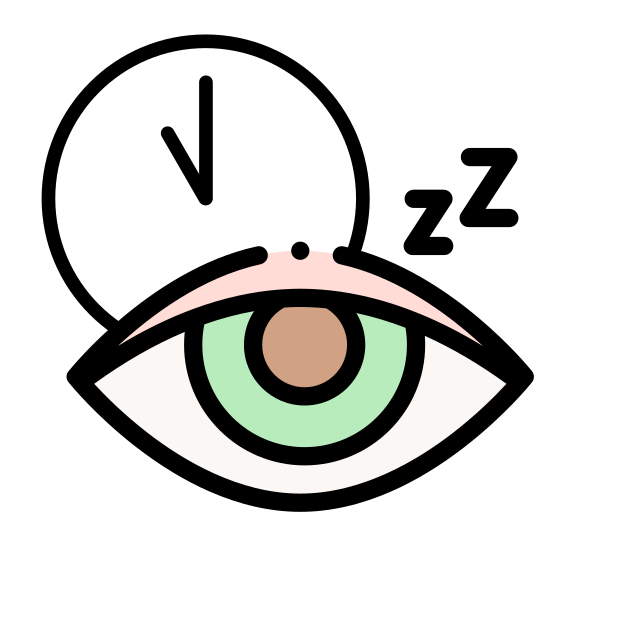
\includegraphics[width=0.33\linewidth]{downloadFigs4latex_NIMH_Applet_Codebook/morning_close_eyes_headerImg} \end{flushleft}

\textbf{Responses}: \emph{Time in HH:MM AM/PM format via clock widget}

\hypertarget{morning_sleep_latency}{%
\section{morning\_sleep\_latency}\label{morning_sleep_latency}}

\textbf{Question}: ``How long did it take you to \textbf{fall asleep}?''

\textbf{Visibility}: \emph{Always}

\textbf{Item Type}: Single-select radio button

\textbf{Header Image}:

\begin{flushleft}
\includegraphics[width=0.33\linewidth]{downloadFigs4latex_NIMH_Applet_Codebook/morning_sleep_latency_headerImg} \end{flushleft}

\textbf{Responses}:

Value

Label

1

less than 5 minutes

2

5 minutes

3

10 minutes

4

15 minutes

5

20 minutes

6

30 minutes

7

40 minutes

8

50 minutes

9

1 hour

10

1 hour 15 minutes

11

1 hour 30 minutes

12

1 hour 45 minutes

13

2 hours

14

more than 2 hours

\hypertarget{morning_wake_number}{%
\section{morning\_wake\_number}\label{morning_wake_number}}

\textbf{Question}: ``How many times did you \textbf{wake up in the night}, not counting your final awakening?''

\textbf{Visibility}: \emph{Always}

\textbf{Item Type}: Single-select radio button

\textbf{Header Image}:

\begin{flushleft}
\includegraphics[width=0.33\linewidth]{downloadFigs4latex_NIMH_Applet_Codebook/morning_wake_number_headerImg} \end{flushleft}

\textbf{Responses}:

Value

Label

1

none

2

once

3

twice

4

3 or more times

\hypertarget{morning_waketime}{%
\section{morning\_waketime}\label{morning_waketime}}

\textbf{Question}: ``What time did you \textbf{wake up} this morning?''

\textbf{Visibility}: \emph{Always}

\textbf{Item Type}: Time input

\textbf{Header Image}:

\begin{flushleft}
\includegraphics[width=0.33\linewidth]{downloadFigs4latex_NIMH_Applet_Codebook/morning_waketime_headerImg} \end{flushleft}

\textbf{Responses}: \emph{Time in HH:MM AM/PM format via clock widget}

\hypertarget{morning_outbed}{%
\section{morning\_outbed}\label{morning_outbed}}

\textbf{Question}: ``What time did you \textbf{get out of bed} for the day?''

\textbf{Visibility}: \emph{Always}

\textbf{Item Type}: Time input

\textbf{Header Image}:

\begin{flushleft}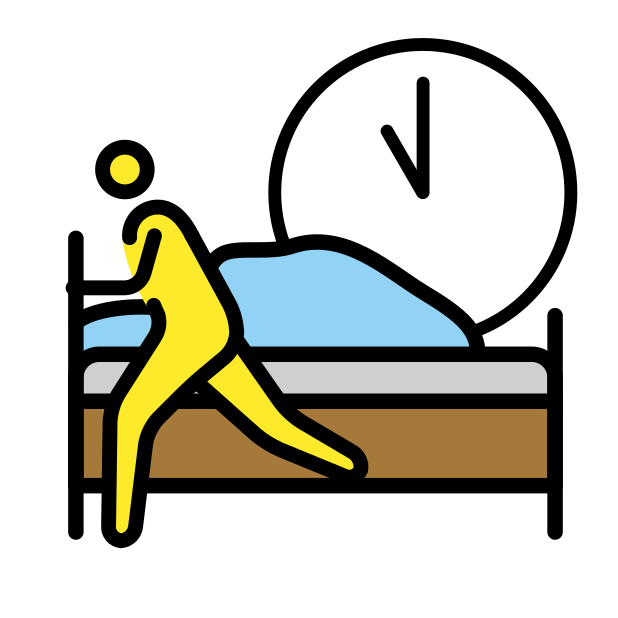
\includegraphics[width=0.33\linewidth]{downloadFigs4latex_NIMH_Applet_Codebook/morning_outbed_headerImg} \end{flushleft}

\textbf{Responses}: \emph{Time in HH:MM AM/PM format via clock widget}

\hypertarget{morning_sleep_quantity}{%
\section{morning\_sleep\_quantity}\label{morning_sleep_quantity}}

\textbf{Question}: ``About how many hours did you \textbf{actually sleep}?''

\textbf{Visibility}: \emph{Always}

\textbf{Item Type}: Single-select radio button

\textbf{Header Image}:

\begin{flushleft}
\includegraphics[width=0.33\linewidth]{downloadFigs4latex_NIMH_Applet_Codebook/morning_sleep_quantity_headerImg} \end{flushleft}

\textbf{Responses}:

Value

Label

1

less than 30 minutes

2

30 minutes

3

1 hour

4

1.5 hours

5

2 hours

6

2.5 hours

7

3 hours

8

3.5 hours

9

4 hours

10

4.5 hours

11

5 hours

12

5.5 hours

13

6 hours

14

6.5 hours

15

7 hours

16

7.5 hours

17

8 hours

18

8.5 hours

19

9 hours

20

9.5 hours

21

10 hours

22

10.5 hours

23

11 hours

24

11.5 hours

25

12 hours

26

12.5 hours

27

13 hours

28

13.5 hours

29

14 hours

30

14.5 hours

31

15 hours

32

15.5 hours

33

16 hours

34

more than 16 hours

\hypertarget{morning_sleep_quality}{%
\section{morning\_sleep\_quality}\label{morning_sleep_quality}}

\textbf{Question}: ``How would you rate the \textbf{quality} of your sleep?''

\textbf{Visibility}: \emph{Always}

\textbf{Item Type}: Slider bar

\textbf{Header Image}: \emph{None}

\textbf{Responses}:

Value

Label

Image

1

very poor

2

2

3

3

4

4

5

5

6

6

7

very good

\hypertarget{morning_sleep_refreshed}{%
\section{morning\_sleep\_refreshed}\label{morning_sleep_refreshed}}

\textbf{Question}: ``How \textbf{refreshed} did you feel when you woke up?''

\textbf{Visibility}: \emph{Always}

\textbf{Item Type}: Slider bar

\textbf{Header Image}: \emph{None}

\textbf{Responses}:

Value

Label

Image

1

not at all refreshed

2

2

3

3

4

4

5

5

6

6

7

fully refreshed

\hypertarget{morning_sleep_problems}{%
\section{morning\_sleep\_problems}\label{morning_sleep_problems}}

\textbf{Question}: ``Which (if any) of the following \textbf{sleep problems} did you have last night?''

\textbf{Visibility}: \emph{Always}

\textbf{Item Type}: Multi-select checkbox

\textbf{Header Image}: \emph{None}

\textbf{Responses}:

Value

Label

Image

1

difficulty falling asleep

2

awakening during the night

3

awakening too early

4

feeling unrefreshed or unrestored despite enough hours of sleep

5

nightmares

6

sleep walking

7

other sleep problem

\hypertarget{morning_sleep_problems_reason}{%
\section{morning\_sleep\_problems\_reason}\label{morning_sleep_problems_reason}}

\textbf{Question}: ``Were the \textbf{sleep problems} due to:''

\textbf{Visibility}: \protect\hyperlink{morning_sleep_problems}{morning\_sleep\_problems}.includes(1) or \protect\hyperlink{morning_sleep_problems}{morning\_sleep\_problems}.includes(2) or \protect\hyperlink{morning_sleep_problems}{morning\_sleep\_problems}.includes(3) or \protect\hyperlink{morning_sleep_problems}{morning\_sleep\_problems}.includes(4) or \protect\hyperlink{morning_sleep_problems}{morning\_sleep\_problems}.includes(5) or \protect\hyperlink{morning_sleep_problems}{morning\_sleep\_problems}.includes(6) or \protect\hyperlink{morning_sleep_problems}{morning\_sleep\_problems}.includes(7)

\textbf{Item Type}: Multi-select checkbox

\textbf{Header Image}: \emph{None}

\textbf{Responses}:

Value

Label

Image

1

noise or other disturbances

2

pain

3

worry

4

other thoughts

5

other reason

\hypertarget{morning_sleeping_pills}{%
\section{morning\_sleeping\_pills}\label{morning_sleeping_pills}}

\textbf{Question}: ``Did you take \textbf{sleeping pills or anything else} to help you sleep last night?''

\textbf{Visibility}: \emph{Always}

\textbf{Item Type}: Single-select radio button

\textbf{Header Image}:

\begin{flushleft}
\includegraphics[width=0.33\linewidth]{downloadFigs4latex_NIMH_Applet_Codebook/morning_sleeping_pills_headerImg} \end{flushleft}

\textbf{Responses}:

Value

Label

1

Yes

0

No

\hypertarget{internetMn_section}{%
\chapter{Internet and Social Media (Morning)}\label{internetMn_section}}

\hypertarget{socialmedia_after_bedtime}{%
\section{socialmedia\_after\_bedtime}\label{socialmedia_after_bedtime}}

\textbf{Question}: ``Were you using your \textbf{social media} accounts \textbf{after bedtime}?''

\textbf{Visibility}: \emph{Always}

\textbf{Item Type}: Single-select radio button

\textbf{Header Image}:

\begin{flushleft}
\includegraphics[width=0.33\linewidth]{downloadFigs4latex_NIMH_Applet_Codebook/socialmedia_after_bedtime_headerImg} \end{flushleft}

\textbf{Responses}:

Value

Label

1

Yes

0

No

\hypertarget{socialmedia_fall_asleep}{%
\section{socialmedia\_fall\_asleep}\label{socialmedia_fall_asleep}}

\textbf{Question}: ``Did your use of social media impact your ability to \textbf{fall asleep} last night?''

\textbf{Visibility}: \emph{Always}

\textbf{Item Type}: Single-select radio button

\textbf{Header Image}:

\begin{flushleft}
\includegraphics[width=0.33\linewidth]{downloadFigs4latex_NIMH_Applet_Codebook/socialmedia_fall_asleep_headerImg} \end{flushleft}

\textbf{Responses}:

Value

Label

1

Yes

0

No

\hypertarget{context_section}{%
\chapter{Context of Assessment}\label{context_section}}

\hypertarget{since_activity_monitor}{%
\section{since\_activity\_monitor}\label{since_activity_monitor}}

\textbf{Question}: ``Have you \textbf{taken your activity monitor off} since your last questionnaire?''

\textbf{Visibility}: \emph{Always}

\textbf{Item Type}: Single-select radio button

\textbf{Header Image}:

\begin{flushleft}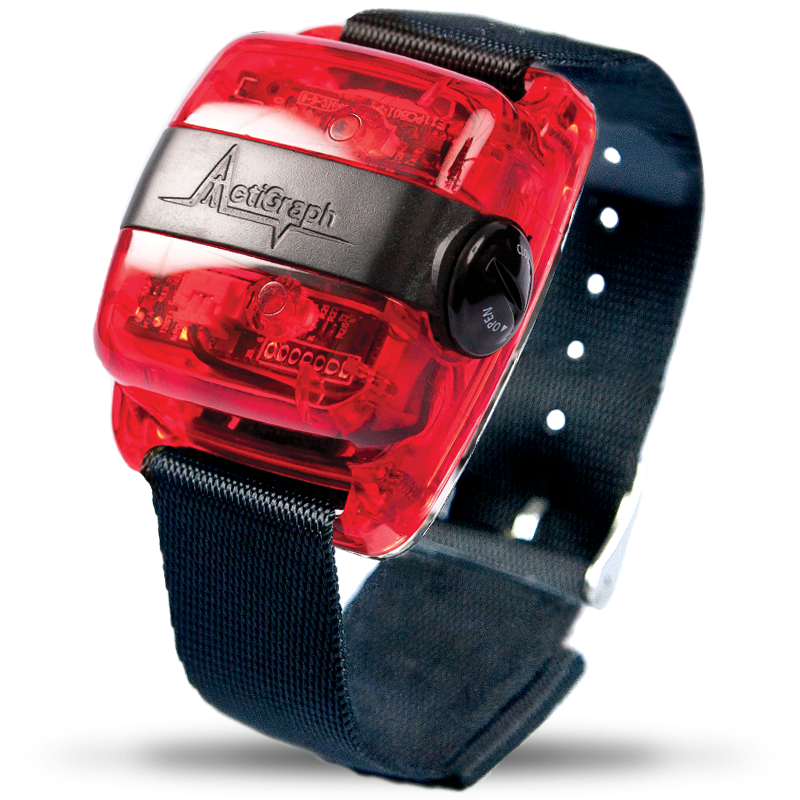
\includegraphics[width=0.33\linewidth]{downloadFigs4latex_NIMH_Applet_Codebook/since_activity_monitor_headerImg} \end{flushleft}

\textbf{Responses}:

Value

Label

1

Yes

0

No

\hypertarget{since_activity_monitor_time}{%
\section{since\_activity\_monitor\_time}\label{since_activity_monitor_time}}

\textbf{Question}: ``When did you \textbf{take it off} and \textbf{put it back on}?''

\textbf{Visibility}: \protect\hyperlink{since_activity_monitor}{since\_activity\_monitor} = 1

\textbf{Item Type}: Time-range input

\textbf{Header Image}:

\begin{flushleft}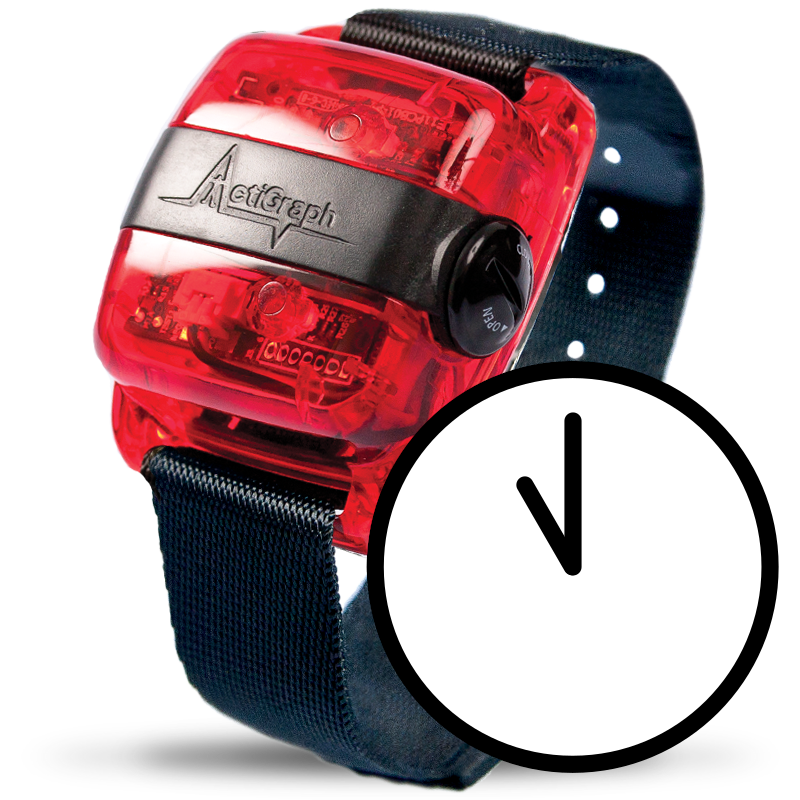
\includegraphics[width=0.33\linewidth]{downloadFigs4latex_NIMH_Applet_Codebook/since_activity_monitor_time_headerImg} \end{flushleft}

\textbf{Responses}: \emph{Time in HH:MM AM/PM format via clock widget}

\hypertarget{now_where}{%
\section{now\_where}\label{now_where}}

\textbf{Question}: ``Where are you \textbf{right now}?''

\textbf{Visibility}: \emph{Always}

\textbf{Item Type}: Single-select radio button

\textbf{Header Image}: \emph{None}

\textbf{Responses}:

Value

Label

Image

1

In my home

2

in home of relative or friend

3

at work or in class

4

in a restaurant/cafe/bar

5

in a store or shop

6

in the gym or fitness center

7

in a hospital or doctor's office

8

in a vehicle (car/bus/etc.)

9

in a public building

10

in a park or garden

11

other place inside

12

other place outside

\hypertarget{since_where}{%
\section{since\_where}\label{since_where}}

\textbf{Question}:

\begin{itemize}
\tightlist
\item
  \emph{Morning Version}: ``Which places have you been \textbf{since you woke up}?''
\item
  \emph{Day/Evening Version}: ``Which places have you been \textbf{since the last questionnaire}?''
\end{itemize}

\textbf{Visibility}: \emph{Always}

\textbf{Item Type}: Multi-select checkbox

\textbf{Header Image}: \emph{None}

\textbf{Responses}:

Value

Label

Image

1

In my home

2

in home of relative or friend

3

at work or in class

4

in a restaurant/cafe/bar

5

in a store or shop

6

in the gym or fitness center

7

in a hospital or doctor's office

8

in a vehicle (car/bus/etc.)

9

in a public building

10

in a park or garden

11

other place inside

12

other place outside

\hypertarget{now_company}{%
\section{now\_company}\label{now_company}}

\textbf{Question}: ``Who is with you at \textbf{this moment}?''

\textbf{Visibility}: \emph{Always}

\textbf{Item Type}: Multi-select checkbox

\textbf{Header Image}: \emph{None}

\textbf{Responses}:

Value

Label

Image

1

no one

2

family member

3

partner/boyfriend/girlfriend

4

friend

5

colleague or classmate

6

stranger

7

a pet

8

other

\hypertarget{since_company}{%
\section{since\_company}\label{since_company}}

\textbf{Question}:

\begin{itemize}
\tightlist
\item
  \emph{Morning Version}: ``Who have you been with \textbf{since you woke up}?''
\item
  \emph{Day/Evening Version}: ``Who have you been with \textbf{since the last questionnaire}?''
\end{itemize}

\textbf{Visibility}: \emph{Always}

\textbf{Item Type}: Multi-select checkbox

\textbf{Header Image}: \emph{None}

\textbf{Responses}:

Value

Label

Image

1

no one

2

family member

3

partner/boyfriend/girlfriend

4

friend

5

colleague or classmate

6

stranger

7

a pet

8

other

\hypertarget{now_activity}{%
\section{now\_activity}\label{now_activity}}

\textbf{Question}: ``What are you doing at \textbf{this moment}?''

\textbf{Visibility}: \emph{Always}

\textbf{Item Type}: Single-select radio button

\textbf{Header Image}: \emph{None}

\textbf{Responses}:

Value

Label

Image

1

nothing or waiting

2

napping/resting

3

eating

4

household chores

5

working (paid or volunteer)

6

homework

7

shopping

8

personal hygiene care

9

physical leisure or sports

10

personal exercise

11

walking the dog

12

traveling or commuting

13

watching tv

14

reading

15

listening to music

16

using a computer/electronic device

17

talking on the phone

18

talking in person

19

texting by phone

20

other nonphysical leisure

21

other activity

\hypertarget{since_activity}{%
\section{since\_activity}\label{since_activity}}

\textbf{Question}:

\begin{itemize}
\tightlist
\item
  \emph{Morning Version}: ``Which of these activities have you done \textbf{since you woke up}?''
\item
  \emph{Day/Evening Version}: ``Which of these activities have you done \textbf{since the last questionnaire}?''
\end{itemize}

\textbf{Visibility}: \emph{Always}

\textbf{Item Type}: Multi-select checkbox

\textbf{Header Image}: \emph{None}

\textbf{Responses}:

Value

Label

Image

1

nothing or waiting

2

napping/resting

3

eating

4

household chores

5

working (paid or volunteer)

6

homework

7

shopping

8

personal hygiene care

9

physical leisure or sports

10

personal exercise

11

walking the dog

12

traveling or commuting

13

watching tv

14

reading

15

listening to music

16

using a computer/electronic device

17

talking on the phone

18

talking in person

19

texting by phone

20

other nonphysical leisure

21

other activity

\hypertarget{mood_section}{%
\chapter{Mood Circumplex and Physical States}\label{mood_section}}

\hypertarget{now_sadness}{%
\section{now\_sadness}\label{now_sadness}}

\textbf{Question}: ``How \textbf{happy versus sad} do you feel right now?''

\textbf{Visibility}: \emph{Always}

\textbf{Item Type}: Slider bar

\textbf{Header Image}: \emph{None}

\textbf{Responses}:

Value

Label

Image

1

very sad/depressed/unhappy

2

2

3

3

4

4

5

5

6

6

7

very cheerful/happy

\hypertarget{now_anxiousness}{%
\section{now\_anxiousness}\label{now_anxiousness}}

\textbf{Question}: ``How \textbf{relaxed versus anxious} do you feel right now?''

\textbf{Visibility}: \emph{Always}

\textbf{Item Type}: Slider bar

\textbf{Header Image}: \emph{None}

\textbf{Responses}:

Value

Label

Image

1

very relaxed/calm

2

2

3

3

4

4

5

5

6

6

7

very nervous/anxious

\hypertarget{now_excited}{%
\section{now\_excited}\label{now_excited}}

\textbf{Question}: ``How \textbf{calm vs.~excited} do you feel right now?''

\textbf{Visibility}: \emph{Always}

\textbf{Item Type}: Slider bar

\textbf{Header Image}: \emph{None}

\textbf{Responses}:

Value

Label

Image

1

calm/quiet

2

2

3

3

4

4

5

5

6

6

7

very excited/aroused

\hypertarget{now_energy}{%
\section{now\_energy}\label{now_energy}}

\textbf{Question}: ``How \textbf{tired vs.~energetic} do you feel right now?''

\textbf{Visibility}: \emph{Always}

\textbf{Item Type}: Slider bar

\textbf{Header Image}: \emph{None}

\textbf{Responses}:

Value

Label

Image

1

very tired/sluggish

2

2

3

3

4

4

5

5

6

6

7

very energetic/lively

\hypertarget{now_distracted}{%
\section{now\_distracted}\label{now_distracted}}

\textbf{Question}: ``How well can you \textbf{concentrate or focus} right now?''

\textbf{Visibility}: \emph{Always}

\textbf{Item Type}: Slider bar

\textbf{Header Image}: \emph{None}

\textbf{Responses}:

Value

Label

Image

1

very focused/attentive

2

2

3

3

4

4

5

5

6

6

7

very unfocused/distracted

\hypertarget{now_irritable}{%
\section{now\_irritable}\label{now_irritable}}

\textbf{Question}: ``How \textbf{irritable or easily angered} do you feel right now?''

\textbf{Visibility}: \emph{Always}

\textbf{Item Type}: Slider bar

\textbf{Header Image}: \emph{None}

\textbf{Responses}:

Value

Label

Image

1

not at all irritable/angry

2

2

3

3

4

4

5

5

6

6

7

very irritable/angry

\hypertarget{now_worried}{%
\section{now\_worried}\label{now_worried}}

\textbf{Question}: ``How \textbf{worried} do you feel right now?''

\textbf{Visibility}: \emph{Always}

\textbf{Item Type}: Slider bar

\textbf{Header Image}: \emph{None}

\textbf{Responses}:

Value

Label

Image

1

not at all worried

2

2

3

3

4

4

5

5

6

6

7

very worried

\hypertarget{now_guilty}{%
\section{now\_guilty}\label{now_guilty}}

\textbf{Question}: ``How \textbf{guilty} do you feel right now?''

\textbf{Visibility}: \emph{Always}

\textbf{Item Type}: Slider bar

\textbf{Header Image}: \emph{None}

\textbf{Responses}:

Value

Label

Image

1

not at all guilty

2

2

3

3

4

4

5

5

6

6

7

very guilty

\hypertarget{now_decisions}{%
\section{now\_decisions}\label{now_decisions}}

\textbf{Question}: ``How well can you make \textbf{decisions} right now?''

\textbf{Visibility}: \emph{Always}

\textbf{Item Type}: Slider bar

\textbf{Header Image}: \emph{None}

\textbf{Responses}:

Value

Label

Image

1

not at all/very indecisive

2

2

3

3

4

4

5

5

6

6

7

very well/very decisve

\hypertarget{now_quick_thinking}{%
\section{now\_quick\_thinking}\label{now_quick_thinking}}

\textbf{Question}: ``How \textbf{quick} is your \textbf{thinking}?''

\textbf{Visibility}: \emph{Always}

\textbf{Item Type}: Slider bar

\textbf{Header Image}: \emph{None}

\textbf{Responses}:

Value

Label

Image

1

slow/cannot think of things

2

2

3

3

4

4

5

5

6

6

7

very quick/lots of ideas

\hypertarget{now_enjoyment}{%
\section{now\_enjoyment}\label{now_enjoyment}}

\textbf{Question}: ``How much are you able to \textbf{enjoy and feel pleasure} in things?''

\textbf{Visibility}: \emph{Always}

\textbf{Item Type}: Slider bar

\textbf{Header Image}: \emph{None}

\textbf{Responses}:

Value

Label

Image

1

no pleasure or enjoyment

2

2

3

3

4

4

5

5

6

6

7

really enjoying things

\hypertarget{now_fidgety}{%
\section{now\_fidgety}\label{now_fidgety}}

\textbf{Question}: ``How \textbf{fidgety or restless} do you feel right now compared to your \textbf{usual self}?''

\textbf{Visibility}: \emph{Always}

\textbf{Item Type}: Slider bar

\textbf{Header Image}: \emph{None}

\textbf{Responses}:

Value

Label

Image

1

not at all restless

2

2

3

3

4

4

5

5

6

6

7

very restless/fidgety/cannot sit still

\hypertarget{now_hungry}{%
\section{now\_hungry}\label{now_hungry}}

\textbf{Question}: ``How \textbf{hungry} do you feel right now?''

\textbf{Visibility}: \emph{Always}

\textbf{Item Type}: Slider bar

\textbf{Header Image}: \emph{None}

\textbf{Responses}:

Value

Label

Image

1

feeling full/not at all hungry

2

2

3

3

4

4

5

5

6

6

7

extremely hungry

\hypertarget{now_sleepy}{%
\section{now\_sleepy}\label{now_sleepy}}

\textbf{Question}: ``How \textbf{sleepy} do you feel right now?''

\textbf{Visibility}: \emph{Always}

\textbf{Item Type}: Slider bar

\textbf{Header Image}: \emph{None}

\textbf{Responses}:

Value

Label

Image

1

not at all sleepy

2

2

3

3

4

4

5

5

6

6

7

very sleepy

\hypertarget{thoughts_section}{%
\chapter{Positive and Negative Thoughts}\label{thoughts_section}}

\hypertarget{now_thoughts_positive}{%
\section{now\_thoughts\_positive}\label{now_thoughts_positive}}

\textbf{Question}: ``To what extent are you having \textbf{positive thoughts}, thinking about nice experiences or things that make you feel good?''

\textbf{Visibility}: \emph{Always}

\textbf{Item Type}: Slider bar

\textbf{Header Image}:

\begin{flushleft}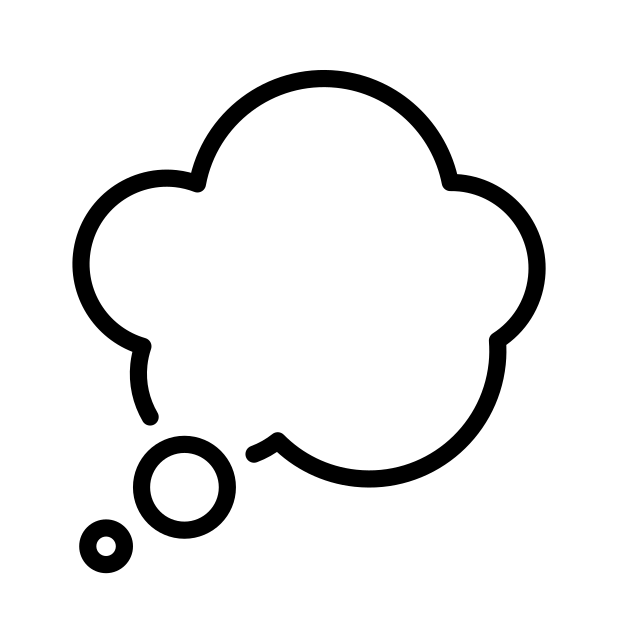
\includegraphics[width=0.33\linewidth]{downloadFigs4latex_NIMH_Applet_Codebook/now_thoughts_positive_headerImg} \end{flushleft}

\textbf{Responses}:

Value

Label

Image

1

not at all

2

2

3

3

4

4

5

5

6

6

7

very frequently

\hypertarget{now_thoughts_negative}{%
\section{now\_thoughts\_negative}\label{now_thoughts_negative}}

\textbf{Question}: ``To what extent are you having \textbf{negative thoughts}, thinking about unpleasant experiences or things that make you feel bad?''

\textbf{Visibility}: \emph{Always}

\textbf{Item Type}: Slider bar

\textbf{Header Image}:

\begin{flushleft}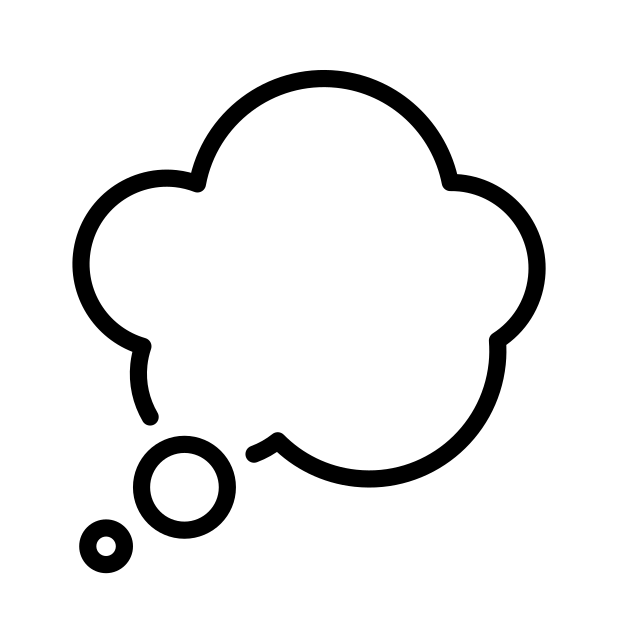
\includegraphics[width=0.33\linewidth]{downloadFigs4latex_NIMH_Applet_Codebook/now_thoughts_negative_headerImg} \end{flushleft}

\textbf{Responses}:

Value

Label

Image

1

not at all

2

2

3

3

4

4

5

5

6

6

7

very frequently

\hypertarget{now_thoughts_negative_about}{%
\section{now\_thoughts\_negative\_about}\label{now_thoughts_negative_about}}

\textbf{Question}: ``Were these thoughts about:''

\textbf{Visibility}: \protect\hyperlink{now_thoughts_negative}{now\_thoughts\_negative} \textgreater{} 1

\textbf{Item Type}: Multi-select checkbox

\textbf{Header Image}:

\begin{flushleft}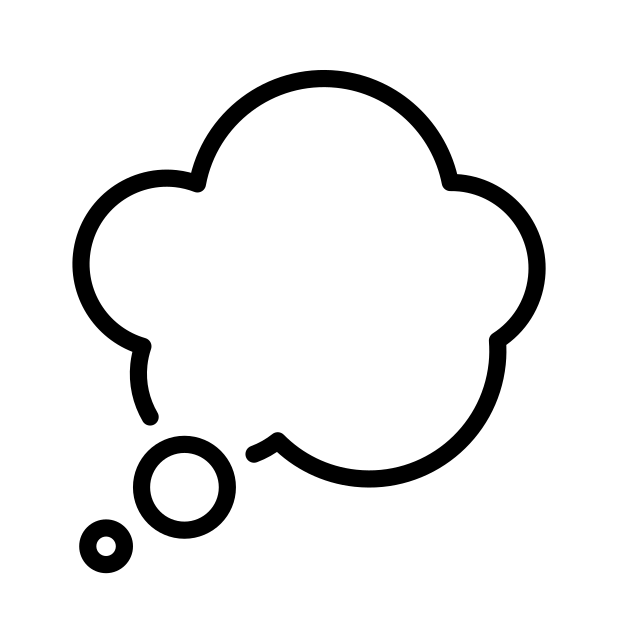
\includegraphics[width=0.33\linewidth]{downloadFigs4latex_NIMH_Applet_Codebook/now_thoughts_negative_about_headerImg} \end{flushleft}

\textbf{Responses}:

Value

Label

Image

1

things you did that you regret

2

things that happened to you or to others

3

worries that you have

4

other negative thoughts

\hypertarget{now_thoughts_negative_severity}{%
\section{now\_thoughts\_negative\_severity}\label{now_thoughts_negative_severity}}

\textbf{Question}: ``How \textbf{severe or disturbing} would you say these thoughts were?''

\textbf{Visibility}: \protect\hyperlink{now_thoughts_negative}{now\_thoughts\_negative} \textgreater{} 1

\textbf{Item Type}: Slider bar

\textbf{Header Image}:

\begin{flushleft}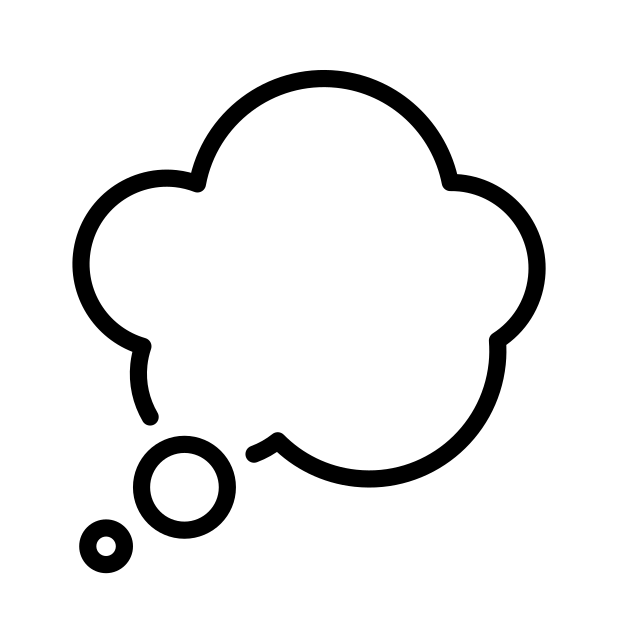
\includegraphics[width=0.33\linewidth]{downloadFigs4latex_NIMH_Applet_Codebook/now_thoughts_negative_severity_headerImg} \end{flushleft}

\textbf{Responses}:

Value

Label

Image

1

not at all severe or disturbing

2

2

3

3

4

4

5

5

6

6

7

very severe or disturbing

\hypertarget{now_thoughts_dangerous}{%
\section{now\_thoughts\_dangerous}\label{now_thoughts_dangerous}}

\textbf{Question}: ``Were these thoughts about things that could be \textbf{dangerous} for you physically?''

\textbf{Visibility}: \protect\hyperlink{now_thoughts_negative_severity}{now\_thoughts\_negative\_severity} \textgreater{} 1

\textbf{Item Type}: Single-select radio button

\textbf{Header Image}:

\begin{flushleft}
\includegraphics[width=0.33\linewidth]{downloadFigs4latex_NIMH_Applet_Codebook/now_thoughts_dangerous_headerImg} \end{flushleft}

\textbf{Responses}:

Value

Label

1

Yes

0

No

\hypertarget{now_thoughts_suicide}{%
\section{now\_thoughts\_suicide}\label{now_thoughts_suicide}}

\textbf{Question}: ``Since the last signal did you have thoughts of harming yourself or of suicide?''

\textbf{Visibility}: \protect\hyperlink{now_thoughts_dangerous}{now\_thoughts\_dangerous} = 1

\textbf{Item Type}: Single-select radio button

\textbf{Header Image}:

\begin{flushleft}
\includegraphics[width=0.33\linewidth]{downloadFigs4latex_NIMH_Applet_Codebook/now_thoughts_suicide_headerImg} \end{flushleft}

\textbf{Responses}:

Value

Label

1

Yes

0

No

\hypertarget{now_thoughts_suicide_warning}{%
\section{now\_thoughts\_suicide\_warning}\label{now_thoughts_suicide_warning}}

\textbf{Question}:

"The information you are providing now is not immediately transmitted to your doctor or to people who can help you.

If you think that you are at the slightest risk of hurting yourself, \textbf{please call the following number now} to talk about it. Someone is available at any time of the day or night:

\textbf{1-800-273-8255}"

\textbf{Visibility}: \protect\hyperlink{now_thoughts_suicide}{now\_thoughts\_suicide} = 1

\textbf{Item Type}: User Message/instructions

\textbf{Header Image}:

\begin{flushleft}
\includegraphics[width=0.33\linewidth]{downloadFigs4latex_NIMH_Applet_Codebook/now_thoughts_suicide_warning_headerImg} \end{flushleft}

\textbf{Responses}: \emph{This item is a markdown message}

\hypertarget{activity_section}{%
\chapter{Physical Activity}\label{activity_section}}

\hypertarget{since_rest}{%
\section{since\_rest}\label{since_rest}}

\textbf{Question}:

\begin{itemize}
\tightlist
\item
  \emph{Morning Version}: ``Since you woke up, did you have a nap or rest?''
\item
  \emph{Day/Evening Version}: ``Since the last questionnaire, did you have a nap or rest?''
\end{itemize}

\textbf{Visibility}: \emph{Always}

\textbf{Item Type}: Single-select radio button

\textbf{Header Image}:

\begin{flushleft}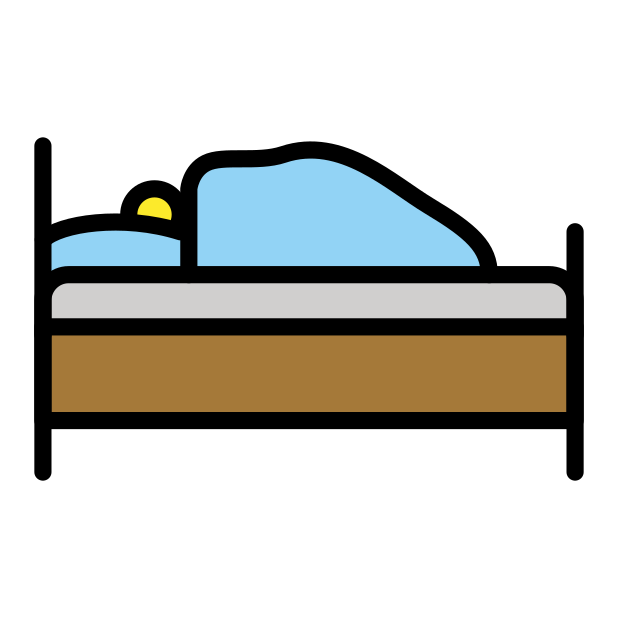
\includegraphics[width=0.33\linewidth]{downloadFigs4latex_NIMH_Applet_Codebook/since_rest_headerImg} \end{flushleft}

\textbf{Responses}:

Value

Label

1

Yes

0

No

\hypertarget{since_rest_duration}{%
\section{since\_rest\_duration}\label{since_rest_duration}}

\textbf{Question}: ``About \textbf{how long} was your nap or rest?''

\textbf{Visibility}: \protect\hyperlink{since_rest}{since\_rest} = 1

\textbf{Item Type}: Single-select radio button

\textbf{Header Image}:

\begin{flushleft}
\includegraphics[width=0.33\linewidth]{downloadFigs4latex_NIMH_Applet_Codebook/since_rest_duration_headerImg} \end{flushleft}

\textbf{Responses}:

Value

Label

1

less than 30 minutes

2

30-60 minutes

3

60-120 minutes

4

longer than 120 minutes

\hypertarget{since_rest_fell_asleep}{%
\section{since\_rest\_fell\_asleep}\label{since_rest_fell_asleep}}

\textbf{Question}: ``Did you actually \textbf{fall asleep} during the nap or rest?''

\textbf{Visibility}: \protect\hyperlink{since_rest}{since\_rest} = 1

\textbf{Item Type}: Single-select radio button

\textbf{Header Image}:

\begin{flushleft}
\includegraphics[width=0.33\linewidth]{downloadFigs4latex_NIMH_Applet_Codebook/since_rest_fell_asleep_headerImg} \end{flushleft}

\textbf{Responses}:

Value

Label

1

Yes

0

No

\hypertarget{since_physical_activity}{%
\section{since\_physical\_activity}\label{since_physical_activity}}

\textbf{Question}:

\begin{itemize}
\tightlist
\item
  \emph{Morning Version}: ``Please select the \textbf{intensity level of activities} you did since you woke up:''
\item
  \emph{Day/Evening Version}: ``Please select the \textbf{intensity level of activities} you did since the last questionnaire:''
\end{itemize}

\textbf{Visibility}: \emph{Always}

\textbf{Item Type}: Multi-select checkbox

\textbf{Header Image}: \emph{None}

\textbf{Responses}:

Value

Label

Image

1

vigorous activities (e.g.~running/fast cycling/heavy lifting or digging)

2

moderate activities (e.g.~tennis/bicycling/carrying light loads)

3

light activities (e.g.~walking/climbing stairs/routine household chores)

\hypertarget{since_vigorous_activity}{%
\section{since\_vigorous\_activity}\label{since_vigorous_activity}}

\textbf{Question}:

\begin{itemize}
\tightlist
\item
  \emph{Morning Version}: ``Since you woke up, how many minutes did you do \textbf{vigorous activities} including intensive sports or exercise (such as running or fast cycling) or intensive physical work (such as heavy lifting or digging)?''
\item
  \emph{Day/Evening Version}: ``Since the last questionnaire, how many minutes did you do \textbf{vigorous activities} including intensive sports or exercise (such as running or fast cycling) or intensive physical work (such as heavy lifting or digging)?''
\end{itemize}

\textbf{Visibility}: \protect\hyperlink{since_physical_activity}{since\_physical\_activity}.includes(1)

\textbf{Item Type}: Single-select radio button

\textbf{Header Image}:

\begin{flushleft}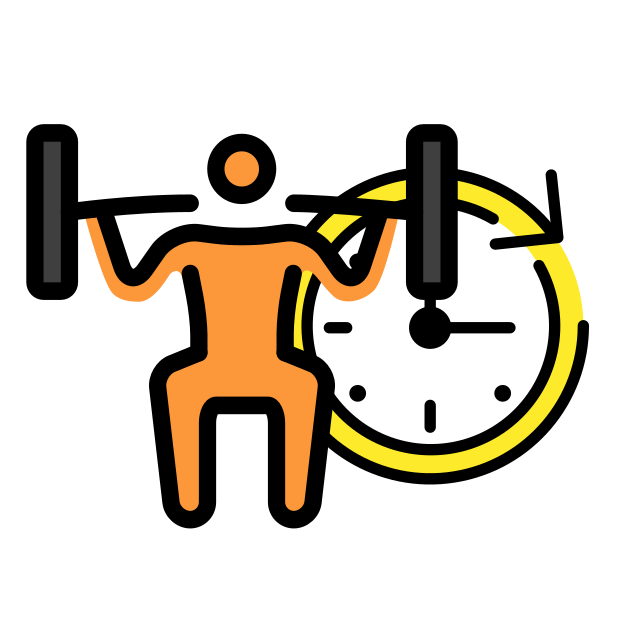
\includegraphics[width=0.33\linewidth]{downloadFigs4latex_NIMH_Applet_Codebook/since_vigorous_activity_headerImg} \end{flushleft}

\textbf{Responses}:

Value

Label

1

5 minutes

2

10 minutes

3

20 minutes

4

30 minutes

5

40 minutes

6

50 minutes

7

60 minutes or more

\hypertarget{since_vigorous_activity_planned}{%
\section{since\_vigorous\_activity\_planned}\label{since_vigorous_activity_planned}}

\textbf{Question}: ``Was this \textbf{vigorous activity} (or activities) part of a \textbf{planned} workout or exercise routine?''

\textbf{Visibility}: \protect\hyperlink{since_physical_activity}{since\_physical\_activity}.includes(1)

\textbf{Item Type}: Single-select radio button

\textbf{Header Image}:

\begin{flushleft}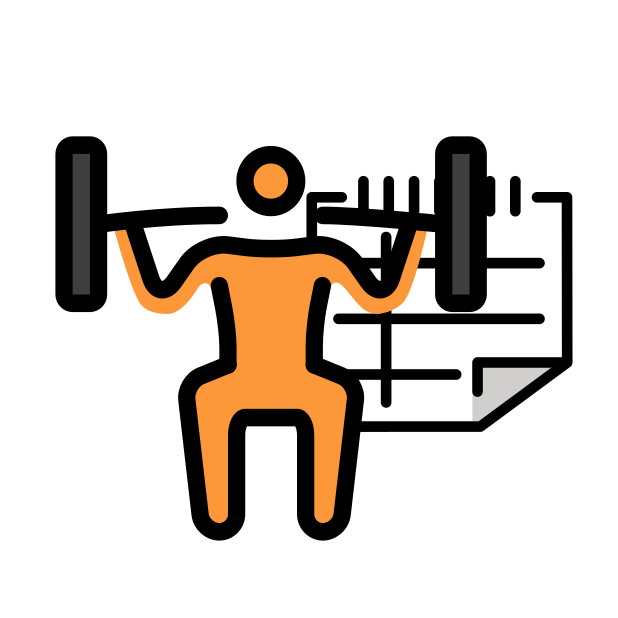
\includegraphics[width=0.33\linewidth]{downloadFigs4latex_NIMH_Applet_Codebook/since_vigorous_activity_planned_headerImg} \end{flushleft}

\textbf{Responses}:

Value

Label

1

Yes

0

No

\hypertarget{since_moderate_activity}{%
\section{since\_moderate\_activity}\label{since_moderate_activity}}

\textbf{Question}:

\begin{itemize}
\tightlist
\item
  \emph{Morning Version}: ``Since you woke up, how many minutes did you do \textbf{moderate activities} (activities that make you breathe somewhat harder than usual such as playing tennis, bicycling, carrying light loads)?''
\item
  \emph{Day/Evening Version}: ``Since the last questionnaire, how many minutes did you do \textbf{moderate activities} (activities that make you breathe somewhat harder than usual such as playing tennis, bicycling, carrying light loads)?''
\end{itemize}

\textbf{Visibility}: \protect\hyperlink{since_physical_activity}{since\_physical\_activity}.includes(2)

\textbf{Item Type}: Single-select radio button

\textbf{Header Image}:

\begin{flushleft}
\includegraphics[width=0.33\linewidth]{downloadFigs4latex_NIMH_Applet_Codebook/since_moderate_activity_headerImg} \end{flushleft}

\textbf{Responses}:

Value

Label

1

5 minutes

2

10 minutes

3

20 minutes

4

30 minutes

5

40 minutes

6

50 minutes

7

60 minutes or more

\hypertarget{since_moderate_activity_planned}{%
\section{since\_moderate\_activity\_planned}\label{since_moderate_activity_planned}}

\textbf{Question}: ``Was this \textbf{moderate activity} (or activities) part of a \textbf{planned} workout or exercise routine?''

\textbf{Visibility}: \protect\hyperlink{since_physical_activity}{since\_physical\_activity}.includes(2)

\textbf{Item Type}: Single-select radio button

\textbf{Header Image}:

\begin{flushleft}
\includegraphics[width=0.33\linewidth]{downloadFigs4latex_NIMH_Applet_Codebook/since_moderate_activity_planned_headerImg} \end{flushleft}

\textbf{Responses}:

Value

Label

1

Yes

0

No

\hypertarget{since_light_activity}{%
\section{since\_light\_activity}\label{since_light_activity}}

\textbf{Question}:

\begin{itemize}
\tightlist
\item
  \emph{Morning Version}: ``Since you woke up, how many minutes did you do \textbf{light activities} (activities that may not make you breathe somewhat harder than usual such as walking, climbing stairs, routine household chores, etc.)?''
\item
  \emph{Day/Evening Version}: ``Since the last questionnaire, how many minutes did you do \textbf{light activities} (activities that may not make you breathe somewhat harder than usual such as walking, climbing stairs, routine household chores, etc.)?''
\end{itemize}

\textbf{Visibility}: \protect\hyperlink{since_physical_activity}{since\_physical\_activity}.includes(3)

\textbf{Item Type}: Single-select radio button

\textbf{Header Image}:

\begin{flushleft}
\includegraphics[width=0.33\linewidth]{downloadFigs4latex_NIMH_Applet_Codebook/since_light_activity_headerImg} \end{flushleft}

\textbf{Responses}:

Value

Label

1

5 minutes

2

10 minutes

3

20 minutes

4

30 minutes

5

40 minutes

6

50 minutes

7

60 minutes or more

\hypertarget{since_light_activity_planned}{%
\section{since\_light\_activity\_planned}\label{since_light_activity_planned}}

\textbf{Question}: ``Was this \textbf{light activity} (or activities) part of a \textbf{planned} workout or exercise routine?''

\textbf{Visibility}: \protect\hyperlink{since_physical_activity}{since\_physical\_activity}.includes(3)

\textbf{Item Type}: Single-select radio button

\textbf{Header Image}:

\begin{flushleft}
\includegraphics[width=0.33\linewidth]{downloadFigs4latex_NIMH_Applet_Codebook/since_light_activity_planned_headerImg} \end{flushleft}

\textbf{Responses}:

Value

Label

1

Yes

0

No

\hypertarget{intake_section}{%
\chapter{Intake: Food/drink/substances}\label{intake_section}}

\hypertarget{since_had_drink}{%
\section{since\_had\_drink}\label{since_had_drink}}

\textbf{Question}:

\begin{itemize}
\tightlist
\item
  \emph{Morning Version}: ``Since you woke up, did you drink:''
\item
  \emph{Day/Evening Version}: ``Since the last questionnaire, did you drink:''
\end{itemize}

\textbf{Visibility}: \emph{Always}

\textbf{Item Type}: Multi-select checkbox

\textbf{Header Image}: \emph{None}

\textbf{Responses}:

Value

Label

Image

1

water

2

milk

3

a caffeinated beverage (like coffee/tea/soda etc.)

4

an alcoholic beverage (wine/beer/liquor etc.)

5

a beverage containing sugar like juice or caffeine-free soda

6

another type of drink

1

water

2

milk

3

a caffeinated beverage (like coffee/tea/soda etc.)

4

an alcoholic beverage (wine/beer/liquor etc.)

5

a beverage containing sugar like juice or caffeine-free soda

6

another type of drink

7

none

\hypertarget{since_had_drink_water_quantity}{%
\section{since\_had\_drink\_water\_quantity}\label{since_had_drink_water_quantity}}

\textbf{Question}: ``How many 8 oz glasses of \textbf{water} did you consume?''

\textbf{Visibility}: \protect\hyperlink{since_had_drink}{since\_had\_drink}.includes(1)

\textbf{Item Type}: Single-select radio button

\textbf{Header Image}:

\begin{flushleft}
\includegraphics[width=0.33\linewidth]{downloadFigs4latex_NIMH_Applet_Codebook/since_had_drink_water_quantity_headerImg} \end{flushleft}

\textbf{Responses}:

Value

Label

1

1 glass

2

2 glasses

3

3 glasses

4

4 glasses

5

5 or more glasses

\hypertarget{since_had_drink_milk_quantity}{%
\section{since\_had\_drink\_milk\_quantity}\label{since_had_drink_milk_quantity}}

\textbf{Question}: ``How many 8 oz glasses of \textbf{milk} did you consume?''

\textbf{Visibility}: \protect\hyperlink{since_had_drink}{since\_had\_drink}.includes(2)

\textbf{Item Type}: Single-select radio button

\textbf{Header Image}:

\begin{flushleft}
\includegraphics[width=0.33\linewidth]{downloadFigs4latex_NIMH_Applet_Codebook/since_had_drink_milk_quantity_headerImg} \end{flushleft}

\textbf{Responses}:

Value

Label

1

1 glass

2

2 glasses

3

3 glasses

4

4 glasses

5

5 or more glasses

\hypertarget{since_had_drink_caffeinated_type}{%
\section{since\_had\_drink\_caffeinated\_type}\label{since_had_drink_caffeinated_type}}

\textbf{Question}: ``What type of \textbf{caffeinated beverage} did you consume?''

\textbf{Visibility}: \protect\hyperlink{since_had_drink}{since\_had\_drink}.includes(3)

\textbf{Item Type}: Multi-select checkbox

\textbf{Header Image}:

\begin{flushleft}
\includegraphics[width=0.33\linewidth]{downloadFigs4latex_NIMH_Applet_Codebook/since_had_drink_caffeinated_type_headerImg} \end{flushleft}

\textbf{Responses}:

Value

Label

Image

1

soda (coke/pepsi/other caffeinated soda)

2

energy drink

3

coffee

4

tea

5

other

\hypertarget{since_had_drink_caffeinated_quantity}{%
\section{since\_had\_drink\_caffeinated\_quantity}\label{since_had_drink_caffeinated_quantity}}

\textbf{Question}: ``How many 8 oz glasses of \textbf{caffeinated drinks} did you consume?''

\textbf{Visibility}: \protect\hyperlink{since_had_drink}{since\_had\_drink}.includes(3)

\textbf{Item Type}: Single-select radio button

\textbf{Header Image}:

\begin{flushleft}
\includegraphics[width=0.33\linewidth]{downloadFigs4latex_NIMH_Applet_Codebook/since_had_drink_caffeinated_quantity_headerImg} \end{flushleft}

\textbf{Responses}:

Value

Label

1

1 glass

2

2 glasses

3

3 glasses

4

4 glasses

5

5 or more glasses

\hypertarget{since_had_drink_alcohol_type}{%
\section{since\_had\_drink\_alcohol\_type}\label{since_had_drink_alcohol_type}}

\textbf{Question}: ``What type of \textbf{alcoholic beverage} did you consume?''

\textbf{Visibility}: \protect\hyperlink{since_had_drink}{since\_had\_drink}.includes(4)

\textbf{Item Type}: Multi-select checkbox

\textbf{Header Image}:

\begin{flushleft}
\includegraphics[width=0.33\linewidth]{downloadFigs4latex_NIMH_Applet_Codebook/since_had_drink_alcohol_type_headerImg} \end{flushleft}

\textbf{Responses}:

Value

Label

Image

1

red wine

2

white wine

3

champagne/sparkling wine

4

beer

5

cocktail

6

whisky or other strong alcohol

7

other type of alcoholic drink

\hypertarget{since_had_drink_alcohol_quantity}{%
\section{since\_had\_drink\_alcohol\_quantity}\label{since_had_drink_alcohol_quantity}}

\textbf{Question}: ``How many servings of \textbf{alcohol} did you consume?''

\textbf{Visibility}: \protect\hyperlink{since_had_drink}{since\_had\_drink}.includes(4)

\textbf{Item Type}: Single-select radio button

\textbf{Header Image}:

\begin{flushleft}
\includegraphics[width=0.33\linewidth]{downloadFigs4latex_NIMH_Applet_Codebook/since_had_drink_alcohol_quantity_headerImg} \end{flushleft}

\textbf{Responses}:

Value

Label

1

1 drink

2

2 drinks

3

3 drinks

4

4 drinks

5

5 or more drinks

\hypertarget{since_had_drink_sugar_quantity}{%
\section{since\_had\_drink\_sugar\_quantity}\label{since_had_drink_sugar_quantity}}

\textbf{Question}: ``How many 8 oz glasses of \textbf{high-sugar drinks} (e.g., juice, soda, some coffee beverages) did you consume?''

\textbf{Visibility}: \protect\hyperlink{since_had_drink}{since\_had\_drink}.includes(5)

\textbf{Item Type}: Single-select radio button

\textbf{Header Image}:

\begin{flushleft}
\includegraphics[width=0.33\linewidth]{downloadFigs4latex_NIMH_Applet_Codebook/since_had_drink_sugar_quantity_headerImg} \end{flushleft}

\textbf{Responses}:

Value

Label

1

1 glass

2

2 glasses

3

3 glasses

4

4 glasses

5

5 or more glasses

\hypertarget{since_eaten_amount}{%
\section{since\_eaten\_amount}\label{since_eaten_amount}}

\textbf{Question}:

\begin{itemize}
\tightlist
\item
  \emph{Morning Version}: ``Since you woke up, which of the following did you have?''
\item
  \emph{Day/Evening Version}: ``Since the last questionnaire, which of the following did you have?''
\end{itemize}

\textbf{Visibility}: \emph{Always}

\textbf{Item Type}: Multi-select checkbox

\textbf{Header Image}: \emph{None}

\textbf{Responses}:

Value

Label

Image

1

snacks

2

small meals

3

regular/full meals

4

large meals

\hypertarget{since_eaten_snacks_quantity}{%
\section{since\_eaten\_snacks\_quantity}\label{since_eaten_snacks_quantity}}

\textbf{Question}: ``How many \textbf{snacks} did you have?''

\textbf{Visibility}: \protect\hyperlink{since_eaten_amount}{since\_eaten\_amount}.includes(1)

\textbf{Item Type}: Single-select radio button

\textbf{Header Image}:

\begin{flushleft}
\includegraphics[width=0.33\linewidth]{downloadFigs4latex_NIMH_Applet_Codebook/since_eaten_snacks_quantity_headerImg} \end{flushleft}

\textbf{Responses}:

Value

Label

1

1 snack

2

2 snacks

3

3 snacks

4

4 snacks

5

5 snacks

6

6 snacks

7

7 snacks

8

8 snacks

9

9 snacks

10

10 snacks

11

more than 10 snacks

\hypertarget{since_eaten_small_meal_quantity}{%
\section{since\_eaten\_small\_meal\_quantity}\label{since_eaten_small_meal_quantity}}

\textbf{Question}: ``How many \textbf{small meals} did you have?''

\textbf{Visibility}: \protect\hyperlink{since_eaten_amount}{since\_eaten\_amount}.includes(2)

\textbf{Item Type}: Single-select radio button

\textbf{Header Image}:

\begin{flushleft}
\includegraphics[width=0.33\linewidth]{downloadFigs4latex_NIMH_Applet_Codebook/since_eaten_small_meal_quantity_headerImg} \end{flushleft}

\textbf{Responses}:

Value

Label

1

1 small meal

2

2 small meals

3

3 small meals

4

4 small meals

5

5 small meals

6

more than 5 small meals

\hypertarget{since_eaten_regular_meal_quantity}{%
\section{since\_eaten\_regular\_meal\_quantity}\label{since_eaten_regular_meal_quantity}}

\textbf{Question}: ``How many \textbf{regular/full meals} did you have?''

\textbf{Visibility}: \protect\hyperlink{since_eaten_amount}{since\_eaten\_amount}.includes(3)

\textbf{Item Type}: Single-select radio button

\textbf{Header Image}:

\begin{flushleft}
\includegraphics[width=0.33\linewidth]{downloadFigs4latex_NIMH_Applet_Codebook/since_eaten_regular_meal_quantity_headerImg} \end{flushleft}

\textbf{Responses}:

Value

Label

1

1 full meal

2

2 full meals

3

3 full meals

4

more than 3 full meals

\hypertarget{since_eaten_large_meal_quantity}{%
\section{since\_eaten\_large\_meal\_quantity}\label{since_eaten_large_meal_quantity}}

\textbf{Question}: ``How many \textbf{large meals} did you have?''

\textbf{Visibility}: \protect\hyperlink{since_eaten_amount}{since\_eaten\_amount}.includes(4)

\textbf{Item Type}: Single-select radio button

\textbf{Header Image}:

\begin{flushleft}
\includegraphics[width=0.33\linewidth]{downloadFigs4latex_NIMH_Applet_Codebook/since_eaten_large_meal_quantity_headerImg} \end{flushleft}

\textbf{Responses}:

Value

Label

1

1 large meal

2

2 large meals

3

more than 2 large meals

\hypertarget{since_eaten_when}{%
\section{since\_eaten\_when}\label{since_eaten_when}}

\textbf{Question}: ``About \textbf{what time} did you eat your largest snack/meal?''

\textbf{Visibility}: \protect\hyperlink{since_eaten_amount}{since\_eaten\_amount}.includes(1) or \protect\hyperlink{since_eaten_amount}{since\_eaten\_amount}.includes(2) or \protect\hyperlink{since_eaten_amount}{since\_eaten\_amount}.includes(3) or \protect\hyperlink{since_eaten_amount}{since\_eaten\_amount}.includes(4)

\textbf{Item Type}: Time input

\textbf{Header Image}:

\begin{flushleft}
\includegraphics[width=0.33\linewidth]{downloadFigs4latex_NIMH_Applet_Codebook/since_eaten_when_headerImg} \end{flushleft}

\textbf{Responses}: \emph{Time in HH:MM AM/PM format via clock widget}

\hypertarget{since_eaten_duration}{%
\section{since\_eaten\_duration}\label{since_eaten_duration}}

\textbf{Question}: ``For \textbf{how long} did you eat in total?''

\textbf{Visibility}: \protect\hyperlink{since_eaten_amount}{since\_eaten\_amount}.includes(1) or \protect\hyperlink{since_eaten_amount}{since\_eaten\_amount}.includes(2) or \protect\hyperlink{since_eaten_amount}{since\_eaten\_amount}.includes(3) or \protect\hyperlink{since_eaten_amount}{since\_eaten\_amount}.includes(4)

\textbf{Item Type}: Single-select radio button

\textbf{Header Image}:

\begin{flushleft}
\includegraphics[width=0.33\linewidth]{downloadFigs4latex_NIMH_Applet_Codebook/since_eaten_duration_headerImg} \end{flushleft}

\textbf{Responses}:

Value

Label

1

5 minutes or less

2

10 minutes

3

15 minutes

4

30 minutes

5

45 minutes

6

1 hour

7

1 hour 30 minutes

8

2 hours or more

\hypertarget{since_eaten_type}{%
\section{since\_eaten\_type}\label{since_eaten_type}}

\textbf{Question}:

\begin{itemize}
\tightlist
\item
  \emph{Morning Version}: ``Please think about all the foods you ate since you woke up. Please select \textbf{all types} of food you ate:''
\item
  \emph{Day/Evening Version}: ``Please think about all the foods you ate since the last questionnaire. Please select \textbf{all types} of food you ate:''
\end{itemize}

\textbf{Visibility}: \protect\hyperlink{since_eaten_amount}{since\_eaten\_amount}.includes(1) or \protect\hyperlink{since_eaten_amount}{since\_eaten\_amount}.includes(2) or \protect\hyperlink{since_eaten_amount}{since\_eaten\_amount}.includes(3) or \protect\hyperlink{since_eaten_amount}{since\_eaten\_amount}.includes(4)

\textbf{Item Type}: Multi-select checkbox

\textbf{Header Image}: \emph{None}

\textbf{Responses}:

Value

Label

Image

1

beef/pork/lamb

2

chicken or other poultry

3

eggs

4

fish

5

dairy (yogurt/milk/cheese)

6

bread/pasta/cereal/other starchy food

7

fruits

8

vegetables

9

sweet foods or candy

10

energy bars

11

potato chips or other salty snacks

12

other

\hypertarget{since_eaten_chocolate}{%
\section{since\_eaten\_chocolate}\label{since_eaten_chocolate}}

\textbf{Question}: ``Did you eat chocolate?''

\textbf{Visibility}: \protect\hyperlink{since_eaten_type}{since\_eaten\_type}.includes(9)

\textbf{Item Type}: Single-select radio button

\textbf{Header Image}:

\begin{flushleft}
\includegraphics[width=0.33\linewidth]{downloadFigs4latex_NIMH_Applet_Codebook/since_eaten_chocolate_headerImg} \end{flushleft}

\textbf{Responses}:

Value

Label

1

Yes

0

No

\hypertarget{since_substances}{%
\section{since\_substances}\label{since_substances}}

\textbf{Question}:

\begin{itemize}
\tightlist
\item
  \emph{Morning Version}: ``Since you woke up, which of the following did you use?''
\item
  \emph{Day/Evening Version}: ``Since the last questionnaire, which of the following did you use?''
\end{itemize}

\textbf{Visibility}: \emph{Always}

\textbf{Item Type}: Multi-select checkbox

\textbf{Header Image}: \emph{None}

\textbf{Responses}:

Value

Label

Image

1

cigarettes

2

cannabis/pot

3

other drug

\hypertarget{since_substances_cigarettes}{%
\section{since\_substances\_cigarettes}\label{since_substances_cigarettes}}

\textbf{Question}: ``How many \textbf{cigarettes} did you have?''

\textbf{Visibility}: \protect\hyperlink{since_substances}{since\_substances}.includes(1)

\textbf{Item Type}: Single-select radio button

\textbf{Header Image}:

\begin{flushleft}
\includegraphics[width=0.33\linewidth]{downloadFigs4latex_NIMH_Applet_Codebook/since_substances_cigarettes_headerImg} \end{flushleft}

\textbf{Responses}:

Value

Label

1

1 cigarette

2

2 cigarettes

3

3 cigarettes

4

4 cigarettes

5

5 cigarettes

6

6-10 cigarettes

7

10-20 cigarettes

8

over 20 cigarettes

\hypertarget{since_substances_cannabis}{%
\section{since\_substances\_cannabis}\label{since_substances_cannabis}}

\textbf{Question}: ``How many \textbf{joints (of cannabis/pot)} did you have?''

\textbf{Visibility}: \protect\hyperlink{since_substances}{since\_substances}.includes(2)

\textbf{Item Type}: Single-select radio button

\textbf{Header Image}:

\begin{flushleft}
\includegraphics[width=0.33\linewidth]{downloadFigs4latex_NIMH_Applet_Codebook/since_substances_cannabis_headerImg} \end{flushleft}

\textbf{Responses}:

Value

Label

1

1 joint

2

2 joints

3

3 joints

4

4 joints

5

5 joints or more

\hypertarget{since_substances_other}{%
\section{since\_substances\_other}\label{since_substances_other}}

\textbf{Question}: ``What \textbf{other drug} did you use?''

\textbf{Visibility}: \protect\hyperlink{since_substances}{since\_substances}.includes(3)

\textbf{Item Type}: Single-select radio button

\textbf{Header Image}: \emph{None}

\textbf{Responses}:

Value

Label

Image

1

cocaine

2

tranquilizers

3

stimulants

4

heroin or other opiate

5

other drug

\hypertarget{events_section}{%
\chapter{Life Events}\label{events_section}}

\hypertarget{event_instructions}{%
\section{event\_instructions}\label{event_instructions}}

\textbf{Question}:

\begin{itemize}
\tightlist
\item
  \emph{Morning Version}: ``Since you woke up, please think of the \textbf{ONE event that affected you the most} (positively or negatively), no matter how slightly.''
\item
  \emph{Day/Evening Version}: ``Since the last questionnaire, please think of the \textbf{ONE event that affected you the most} (positively or negatively), no matter how slightly.''
\end{itemize}

\textbf{Visibility}: \emph{Always}

\textbf{Item Type}: User Message/instructions

\textbf{Header Image}:

\begin{flushleft}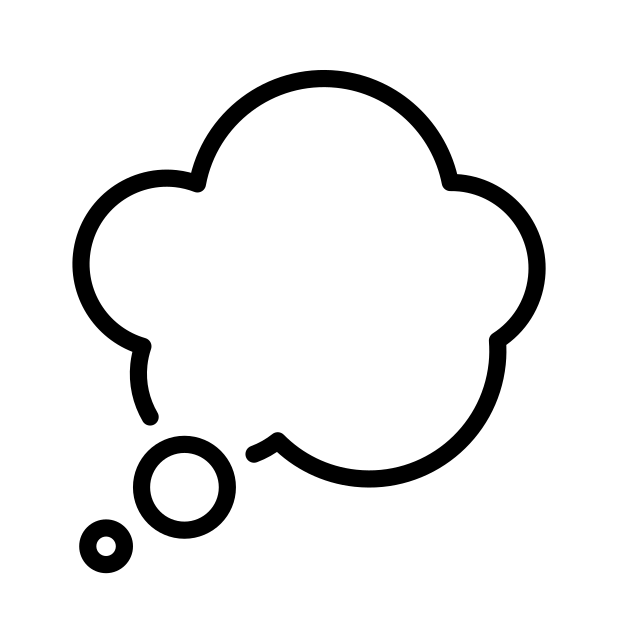
\includegraphics[width=0.33\linewidth]{downloadFigs4latex_NIMH_Applet_Codebook/event_instructions_headerImg} \end{flushleft}

\textbf{Responses}: \emph{This item is a markdown message}

\hypertarget{event_category}{%
\section{event\_category}\label{event_category}}

\textbf{Question}: ``Which of the \textbf{following categories} best describes the area of your life in which the \textbf{event occurred}?''

\textbf{Visibility}: \emph{Always}

\textbf{Item Type}: Single-select radio button

\textbf{Header Image}:

\begin{flushleft}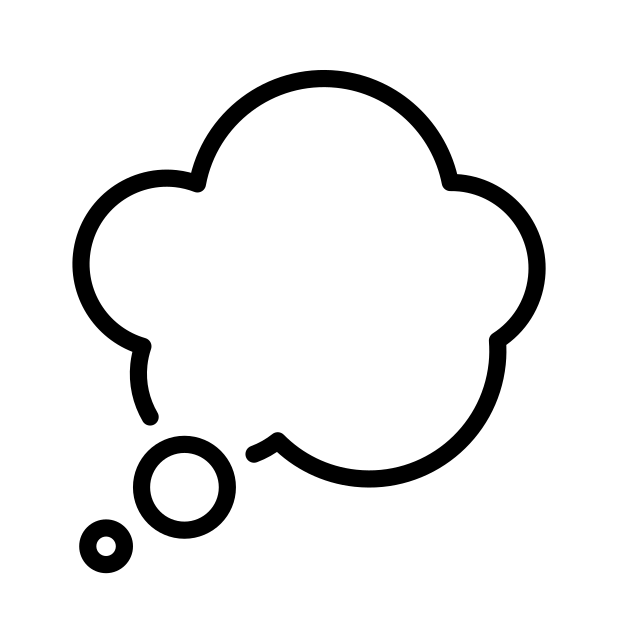
\includegraphics[width=0.33\linewidth]{downloadFigs4latex_NIMH_Applet_Codebook/event_category_headerImg} \end{flushleft}

\textbf{Responses}:

Value

Label

Image

1

work

2

education

3

family or friend relationships

4

interactions with colleagues

5

interactions with strangers

6

housing or residence

7

leisure

8

exercise

9

health

10

finances

11

religion or spirituality

12

legal or judicial

13

traveling or commuting

14

other

\hypertarget{event_impact_positive}{%
\section{event\_impact\_positive}\label{event_impact_positive}}

\textbf{Question}: ``To what degree did this event have a \textbf{positive impact} on you?''

\textbf{Visibility}: \emph{Always}

\textbf{Item Type}: Slider bar

\textbf{Header Image}:

\begin{flushleft}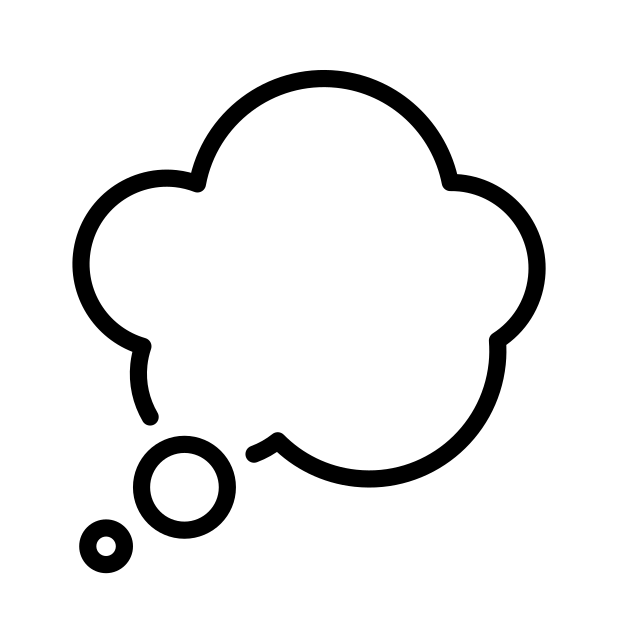
\includegraphics[width=0.33\linewidth]{downloadFigs4latex_NIMH_Applet_Codebook/event_impact_positive_headerImg} \end{flushleft}

\textbf{Responses}:

Value

Label

Image

1

no positive impact

2

2

3

3

4

4

5

5

6

6

7

extremely positive

\hypertarget{event_impact_negative}{%
\section{event\_impact\_negative}\label{event_impact_negative}}

\textbf{Question}: ``To what degree did this event have a \textbf{negative impact} on you?''

\textbf{Visibility}: \emph{Always}

\textbf{Item Type}: Slider bar

\textbf{Header Image}:

\begin{flushleft}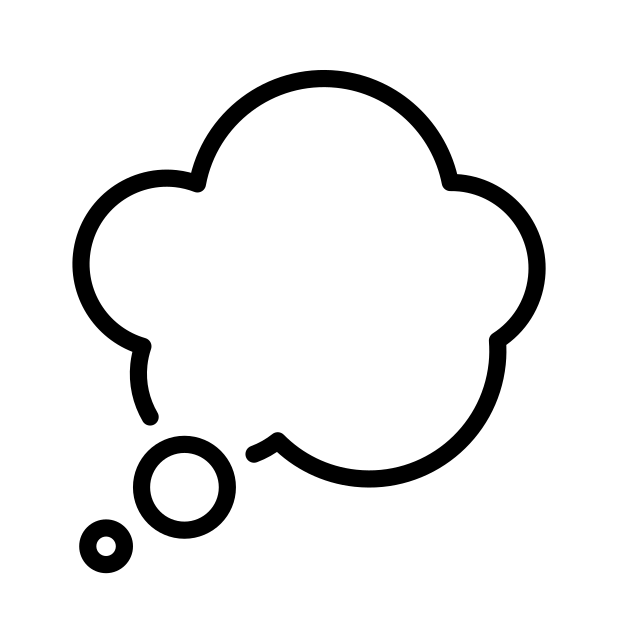
\includegraphics[width=0.33\linewidth]{downloadFigs4latex_NIMH_Applet_Codebook/event_impact_negative_headerImg} \end{flushleft}

\textbf{Responses}:

Value

Label

Image

1

no negative impact

2

2

3

3

4

4

5

5

6

6

7

extremely negative

\hypertarget{event_other}{%
\section{event\_other}\label{event_other}}

\textbf{Question}: ``Did \textbf{more than one event} occur that significantly influenced you?''

\textbf{Visibility}: \emph{Always}

\textbf{Item Type}: Single-select radio button

\textbf{Header Image}:

\begin{flushleft}\includegraphics[width=0.33\linewidth]{downloadFigs4latex_NIMH_Applet_Codebook/event_other_headerImg} \end{flushleft}

\textbf{Responses}:

Value

Label

1

Yes

0

No

\hypertarget{event_other_impact_positive}{%
\section{event\_other\_impact\_positive}\label{event_other_impact_positive}}

\textbf{Question}: ``To what degree did this other event have a \textbf{positive impact} on you?''

\textbf{Visibility}: \protect\hyperlink{event_other}{event\_other} = 1

\textbf{Item Type}: Slider bar

\textbf{Header Image}:

\begin{flushleft}\includegraphics[width=0.33\linewidth]{downloadFigs4latex_NIMH_Applet_Codebook/event_other_impact_positive_headerImg} \end{flushleft}

\textbf{Responses}:

Value

Label

Image

1

no positive impact

2

2

3

3

4

4

5

5

6

6

7

extremely positive

\hypertarget{event_other_impact_negative}{%
\section{event\_other\_impact\_negative}\label{event_other_impact_negative}}

\textbf{Question}: ``To what degree did this other event have a \textbf{negative impact} on you?''

\textbf{Visibility}: \protect\hyperlink{event_other}{event\_other} = 1

\textbf{Item Type}: Slider bar

\textbf{Header Image}:

\begin{flushleft}\includegraphics[width=0.33\linewidth]{downloadFigs4latex_NIMH_Applet_Codebook/event_other_impact_negative_headerImg} \end{flushleft}

\textbf{Responses}:

Value

Label

Image

1

no negative impact

2

2

3

3

4

4

5

5

6

6

7

extremely negative

\hypertarget{pain_section}{%
\chapter{Physical Pain}\label{pain_section}}

\hypertarget{now_pain}{%
\section{now\_pain}\label{now_pain}}

\textbf{Question}: ``Are you in \textbf{pain right now} (other than headache pain)?''

\textbf{Visibility}: \emph{Always}

\textbf{Item Type}: Single-select radio button

\textbf{Header Image}:

\begin{flushleft}\includegraphics[width=0.33\linewidth]{downloadFigs4latex_NIMH_Applet_Codebook/now_pain_headerImg} \end{flushleft}

\textbf{Responses}:

Value

Label

2

Yes

1

No

\hypertarget{now_pain_where}{%
\section{now\_pain\_where}\label{now_pain_where}}

\textbf{Question}: ``\textbf{Where} are you having pain?''

\textbf{Visibility}: \protect\hyperlink{now_pain}{now\_pain} = 2

\textbf{Item Type}: Multi-select checkbox

\textbf{Header Image}:

\begin{flushleft}\includegraphics[width=0.33\linewidth]{downloadFigs4latex_NIMH_Applet_Codebook/now_pain_where_headerImg} \end{flushleft}

\textbf{Responses}:

Value

Label

Image

1

joint/muscle

2

back or neck

3

stomach/bowel

4

other

\hypertarget{now_pain_level}{%
\section{now\_pain\_level}\label{now_pain_level}}

\textbf{Question}: ``How \textbf{severe} is your pain right now?''

\textbf{Visibility}: \protect\hyperlink{now_pain}{now\_pain} = 2

\textbf{Item Type}: Slider bar

\textbf{Header Image}:

\begin{flushleft}\includegraphics[width=0.33\linewidth]{downloadFigs4latex_NIMH_Applet_Codebook/now_pain_level_headerImg} \end{flushleft}

\textbf{Responses}:

Value

Label

Image

1

very minor pain

2

2

3

3

4

4

5

5

6

6

7

extreme pain

\hypertarget{since_pain}{%
\section{since\_pain}\label{since_pain}}

\textbf{Question}:

\begin{itemize}
\tightlist
\item
  \emph{Morning Version}: ``Have you experienced any \textbf{pain since you woke up} (other than headache pain)?''
\item
  \emph{Day/Evening Version}: ``Have you experienced any \textbf{pain since the last questionnaire} (other than headache pain)?''
\end{itemize}

\textbf{Visibility}: \protect\hyperlink{now_pain}{now\_pain} = 1

\textbf{Item Type}: Single-select radio button

\textbf{Header Image}:

\begin{flushleft}\includegraphics[width=0.33\linewidth]{downloadFigs4latex_NIMH_Applet_Codebook/since_pain_headerImg} \end{flushleft}

\textbf{Responses}:

Value

Label

2

Yes

1

No

\hypertarget{since_pain_where}{%
\section{since\_pain\_where}\label{since_pain_where}}

\textbf{Question}: ``\textbf{Where} did this pain occur?''

\textbf{Visibility}: \protect\hyperlink{since_pain}{since\_pain} = 2

\textbf{Item Type}: Multi-select checkbox

\textbf{Header Image}:

\begin{flushleft}\includegraphics[width=0.33\linewidth]{downloadFigs4latex_NIMH_Applet_Codebook/since_pain_where_headerImg} \end{flushleft}

\textbf{Responses}:

Value

Label

Image

1

joint/muscle

2

back or neck

3

stomach/bowel

4

other

\hypertarget{since_pain_level}{%
\section{since\_pain\_level}\label{since_pain_level}}

\textbf{Question}: ``How \textbf{severe} was the pain you experienced since you woke up?''

\textbf{Visibility}: \protect\hyperlink{since_pain}{since\_pain} = 2

\textbf{Item Type}: Slider bar

\textbf{Header Image}:

\begin{flushleft}\includegraphics[width=0.33\linewidth]{downloadFigs4latex_NIMH_Applet_Codebook/since_pain_level_headerImg} \end{flushleft}

\textbf{Responses}:

Value

Label

Image

1

very minor pain

2

2

3

3

4

4

5

5

6

6

7

extreme pain

\hypertarget{headache_section}{%
\chapter{Headache}\label{headache_section}}

\hypertarget{headache}{%
\section{headache}\label{headache}}

\textbf{Question}: ``Have you experienced a \textbf{headache} since the last questionnaire?''

\textbf{Visibility}: \emph{Always}

\textbf{Item Type}: Single-select radio button

\textbf{Header Image}:

\begin{flushleft}\includegraphics[width=0.33\linewidth]{downloadFigs4latex_NIMH_Applet_Codebook/headache_headerImg} \end{flushleft}

\textbf{Responses}:

Value

Label

2

Yes

1

No

\hypertarget{headache_same}{%
\section{headache\_same}\label{headache_same}}

\textbf{Question}: ``Is this the \textbf{same headache} that you reported in the last questionnaire?''

\textbf{Visibility}: \protect\hyperlink{headache}{headache} = 2

\textbf{Item Type}: Single-select radio button

\textbf{Header Image}:

\begin{flushleft}\includegraphics[width=0.33\linewidth]{downloadFigs4latex_NIMH_Applet_Codebook/headache_same_headerImg} \end{flushleft}

\textbf{Responses}:

Value

Label

2

Yes

1

No

\hypertarget{headache_start}{%
\section{headache\_start}\label{headache_start}}

\textbf{Question}: ``What time did the headache \textbf{begin}?''

\textbf{Visibility}: \protect\hyperlink{headache_same}{headache\_same} = 1

\textbf{Item Type}: Time input

\textbf{Header Image}:

\begin{flushleft}\includegraphics[width=0.33\linewidth]{downloadFigs4latex_NIMH_Applet_Codebook/headache_start_headerImg} \end{flushleft}

\textbf{Responses}: \emph{Time in HH:MM AM/PM format via clock widget}

\hypertarget{headache_current}{%
\section{headache\_current}\label{headache_current}}

\textbf{Question}: ``Is this headache \textbf{still present}?''

\textbf{Visibility}: \protect\hyperlink{headache}{headache} = 2

\textbf{Item Type}: Single-select radio button

\textbf{Header Image}:

\begin{flushleft}\includegraphics[width=0.33\linewidth]{downloadFigs4latex_NIMH_Applet_Codebook/headache_current_headerImg} \end{flushleft}

\textbf{Responses}:

Value

Label

2

Yes

1

No

\hypertarget{headache_end}{%
\section{headache\_end}\label{headache_end}}

\textbf{Question}: ``What time did the headache \textbf{end}?''

\textbf{Visibility}: \protect\hyperlink{headache_current}{headache\_current} = 1

\textbf{Item Type}: Time input

\textbf{Header Image}:

\begin{flushleft}\includegraphics[width=0.33\linewidth]{downloadFigs4latex_NIMH_Applet_Codebook/headache_end_headerImg} \end{flushleft}

\textbf{Responses}: \emph{Time in HH:MM AM/PM format via clock widget}

\hypertarget{headache_intensity}{%
\section{headache\_intensity}\label{headache_intensity}}

\textbf{Question}: ``How \textbf{intense} is (or was) the headache?''

\textbf{Visibility}: \protect\hyperlink{headache}{headache} = 2

\textbf{Item Type}: Slider bar

\textbf{Header Image}:

\begin{flushleft}\includegraphics[width=0.33\linewidth]{downloadFigs4latex_NIMH_Applet_Codebook/headache_intensity_headerImg} \end{flushleft}

\textbf{Responses}:

Value

Label

Image

1

very minor

2

2

3

3

4

4

5

5

6

6

7

extremely intense

\hypertarget{headache_sudden}{%
\section{headache\_sudden}\label{headache_sudden}}

\textbf{Question}: ``Did the headache come on \textbf{suddenly}?''

\textbf{Visibility}: \protect\hyperlink{headache}{headache} = 2

\textbf{Item Type}: Single-select radio button

\textbf{Header Image}:

\begin{flushleft}\includegraphics[width=0.33\linewidth]{downloadFigs4latex_NIMH_Applet_Codebook/headache_sudden_headerImg} \end{flushleft}

\textbf{Responses}:

Value

Label

1

Yes

0

No

\hypertarget{headache_trigger}{%
\section{headache\_trigger}\label{headache_trigger}}

\textbf{Question}: ``Did something in particular \textbf{trigger} the headache?''

\textbf{Visibility}: \protect\hyperlink{headache}{headache} = 2

\textbf{Item Type}: Single-select radio button

\textbf{Header Image}:

\begin{flushleft}\includegraphics[width=0.33\linewidth]{downloadFigs4latex_NIMH_Applet_Codebook/headache_trigger_headerImg} \end{flushleft}

\textbf{Responses}:

Value

Label

1

Yes

0

No

\hypertarget{headache_trigger_category}{%
\section{headache\_trigger\_category}\label{headache_trigger_category}}

\textbf{Question}: ``What do you think \textbf{triggered} the headache?''

\textbf{Visibility}: \protect\hyperlink{headache_trigger}{headache\_trigger} = 1

\textbf{Item Type}: Multi-select checkbox

\textbf{Header Image}:

\begin{flushleft}\includegraphics[width=0.33\linewidth]{downloadFigs4latex_NIMH_Applet_Codebook/headache_trigger_category_headerImg} \end{flushleft}

\textbf{Responses}:

Value

Label

Image

1

bright light

2

odor/smell

3

noise

4

food

5

alcoholic drink

6

non-alcoholic beverage

7

hunger

8

thirst/dehydration

9

pain

10

exercise

11

stress

12

other

\hypertarget{headache_location}{%
\section{headache\_location}\label{headache_location}}

\textbf{Question}: ``\textbf{Where} is (or was) the headache?''

\textbf{Visibility}: \protect\hyperlink{headache}{headache} = 2

\textbf{Item Type}: Single-select radio button

\textbf{Header Image}:

\begin{flushleft}\includegraphics[width=0.33\linewidth]{downloadFigs4latex_NIMH_Applet_Codebook/headache_location_headerImg} \end{flushleft}

\textbf{Responses}:

Value

Label

Image

1

both sides of your head

2

left side only

3

right side only

4

moved from one side to another

\hypertarget{headache_pulsating}{%
\section{headache\_pulsating}\label{headache_pulsating}}

\textbf{Question}: ``Is (or was) the pain \textbf{throbbing}, \textbf{beating} or \textbf{pulsating}?''

\textbf{Visibility}: \protect\hyperlink{headache}{headache} = 2

\textbf{Item Type}: Single-select radio button

\textbf{Header Image}:

\begin{flushleft}\includegraphics[width=0.33\linewidth]{downloadFigs4latex_NIMH_Applet_Codebook/headache_pulsating_headerImg} \end{flushleft}

\textbf{Responses}:

Value

Label

1

Yes

0

No

\hypertarget{headache_effort}{%
\section{headache\_effort}\label{headache_effort}}

\textbf{Question}: ``Does (or did) the headache pain \textbf{increase with routine physical activity} such as bending over or climbing stairs?''

\textbf{Visibility}: \protect\hyperlink{headache}{headache} = 2

\textbf{Item Type}: Single-select radio button

\textbf{Header Image}:

\begin{flushleft}\includegraphics[width=0.33\linewidth]{downloadFigs4latex_NIMH_Applet_Codebook/headache_effort_headerImg} \end{flushleft}

\textbf{Responses}:

Value

Label

1

Yes

0

No

\hypertarget{headache_nausea}{%
\section{headache\_nausea}\label{headache_nausea}}

\textbf{Question}: ``Do (or did) you feel \textbf{nauseated}, \textbf{vomit} or have \textbf{diarrhea}?''

\textbf{Visibility}: \protect\hyperlink{headache}{headache} = 2

\textbf{Item Type}: Single-select radio button

\textbf{Header Image}:

\begin{flushleft}\includegraphics[width=0.33\linewidth]{downloadFigs4latex_NIMH_Applet_Codebook/headache_nausea_headerImg} \end{flushleft}

\textbf{Responses}:

Value

Label

1

Yes

0

No

\hypertarget{headache_light}{%
\section{headache\_light}\label{headache_light}}

\textbf{Question}: ``How much does (or did) \textbf{light} bother you?''

\textbf{Visibility}: \protect\hyperlink{headache}{headache} = 2

\textbf{Item Type}: Single-select radio button

\textbf{Header Image}:

\begin{flushleft}\includegraphics[width=0.33\linewidth]{downloadFigs4latex_NIMH_Applet_Codebook/headache_light_headerImg} \end{flushleft}

\textbf{Responses}:

Value

Label

Image

1

not at all

2

mildly

3

moderately

4

severely

\hypertarget{headache_noise}{%
\section{headache\_noise}\label{headache_noise}}

\textbf{Question}: ``How much does (or did) \textbf{noise} such as music, talking, TV, bother you?''

\textbf{Visibility}: \protect\hyperlink{headache}{headache} = 2

\textbf{Item Type}: Single-select radio button

\textbf{Header Image}:

\begin{flushleft}\includegraphics[width=0.33\linewidth]{downloadFigs4latex_NIMH_Applet_Codebook/headache_noise_headerImg} \end{flushleft}

\textbf{Responses}:

Value

Label

Image

1

not at all

2

mildly

3

moderately

4

severely

\hypertarget{headache_smell}{%
\section{headache\_smell}\label{headache_smell}}

\textbf{Question}: ``How much does (or did) \textbf{certain odors} such as perfume, food, smoke, bother you?''

\textbf{Visibility}: \protect\hyperlink{headache}{headache} = 2

\textbf{Item Type}: Single-select radio button

\textbf{Header Image}:

\begin{flushleft}\includegraphics[width=0.33\linewidth]{downloadFigs4latex_NIMH_Applet_Codebook/headache_smell_headerImg} \end{flushleft}

\textbf{Responses}:

Value

Label

Image

1

not at all

2

mildly

3

moderately

4

severely

\hypertarget{headache_vision_changes}{%
\section{headache\_vision\_changes}\label{headache_vision_changes}}

\textbf{Question}: ``Which (if any) of the following \textbf{vision changes} did you experience?''

\textbf{Visibility}: \protect\hyperlink{headache}{headache} = 2

\textbf{Item Type}: Multi-select checkbox

\textbf{Header Image}:

\begin{flushleft}\includegraphics[width=0.33\linewidth]{downloadFigs4latex_NIMH_Applet_Codebook/headache_vision_changes_headerImg} \end{flushleft}

\textbf{Responses}:

Value

Label

Image

1

blurred or distorted vision

2

flashing lights/shapes

3

blind spots or missing parts

\hypertarget{headache_vision_change_time}{%
\section{headache\_vision\_change\_time}\label{headache_vision_change_time}}

\textbf{Question}: ``\textbf{When} did those \textbf{vision changes} occur with respect to the \textbf{onset} of the headache pain?''

\textbf{Visibility}: \protect\hyperlink{headache_vision_changes}{headache\_vision\_changes}.includes(2) or \protect\hyperlink{headache_vision_changes}{headache\_vision\_changes}.includes(3) or \protect\hyperlink{headache_vision_changes}{headache\_vision\_changes}.includes(4)

\textbf{Item Type}: Single-select radio button

\textbf{Header Image}:

\begin{flushleft}\includegraphics[width=0.33\linewidth]{downloadFigs4latex_NIMH_Applet_Codebook/headache_vision_change_time_headerImg} \end{flushleft}

\textbf{Responses}:

Value

Label

Image

1

before headache pain

2

after headache pain

\hypertarget{headache_numbing}{%
\section{headache\_numbing}\label{headache_numbing}}

\textbf{Question}: ``Is (or was) your headache accompanied by any \textbf{numbing or tingling} in certain body areas?''

\textbf{Visibility}: \protect\hyperlink{headache}{headache} = 2

\textbf{Item Type}: Single-select radio button

\textbf{Header Image}:

\begin{flushleft}\includegraphics[width=0.33\linewidth]{downloadFigs4latex_NIMH_Applet_Codebook/headache_numbing_headerImg} \end{flushleft}

\textbf{Responses}:

Value

Label

1

Yes

0

No

\hypertarget{headache_numbing_time}{%
\section{headache\_numbing\_time}\label{headache_numbing_time}}

\textbf{Question}: ``\textbf{When} did this \textbf{numbing or tingling} occur with respect to \textbf{onset} of the headache pain?''

\textbf{Visibility}: \protect\hyperlink{headache_numbing}{headache\_numbing} = 1

\textbf{Item Type}: Single-select radio button

\textbf{Header Image}:

\begin{flushleft}\includegraphics[width=0.33\linewidth]{downloadFigs4latex_NIMH_Applet_Codebook/headache_numbing_time_headerImg} \end{flushleft}

\textbf{Responses}:

Value

Label

Image

1

before headache pain

2

after headache pain

\hypertarget{headache_confusing}{%
\section{headache\_confusing}\label{headache_confusing}}

\textbf{Question}: ``Does (or did) the headache make it \textbf{difficult} to \textbf{speak}, \textbf{think} or \textbf{express yourself}?''

\textbf{Visibility}: \protect\hyperlink{headache}{headache} = 2

\textbf{Item Type}: Single-select radio button

\textbf{Header Image}:

\begin{flushleft}\includegraphics[width=0.33\linewidth]{downloadFigs4latex_NIMH_Applet_Codebook/headache_confusing_headerImg} \end{flushleft}

\textbf{Responses}:

Value

Label

1

Yes

0

No

\hypertarget{headache_confusing_time}{%
\section{headache\_confusing\_time}\label{headache_confusing_time}}

\textbf{Question}: ``When did this \textbf{difficulty} occur with respect to the \textbf{onset} of the headache?''

\textbf{Visibility}: \protect\hyperlink{headache_confusing}{headache\_confusing} = 1

\textbf{Item Type}: Single-select radio button

\textbf{Header Image}:

\begin{flushleft}\includegraphics[width=0.33\linewidth]{downloadFigs4latex_NIMH_Applet_Codebook/headache_confusing_time_headerImg} \end{flushleft}

\textbf{Responses}:

Value

Label

Image

1

before headache pain

2

after headache pain

\hypertarget{headache_medication}{%
\section{headache\_medication}\label{headache_medication}}

\textbf{Question}: ``Which (if any) did you take to \textbf{treat} your headache?''

\textbf{Visibility}: \protect\hyperlink{headache}{headache} = 2

\textbf{Item Type}: Multi-select checkbox

\textbf{Header Image}:

\begin{flushleft}\includegraphics[width=0.33\linewidth]{downloadFigs4latex_NIMH_Applet_Codebook/headache_medication_headerImg} \end{flushleft}

\textbf{Responses}:

Value

Label

Image

1

over-the-counter medications

2

prescription medications

\hypertarget{headache_interference}{%
\section{headache\_interference}\label{headache_interference}}

\textbf{Question}: ``How much does (or did) the headache \textbf{interfere with your activities}?''

\textbf{Visibility}: \protect\hyperlink{headache}{headache} = 2

\textbf{Item Type}: Single-select radio button

\textbf{Header Image}:

\begin{flushleft}\includegraphics[width=0.33\linewidth]{downloadFigs4latex_NIMH_Applet_Codebook/headache_interference_headerImg} \end{flushleft}

\textbf{Responses}:

Value

Label

Image

1

not at all

2

mildly

3

moderately

4

severely

\hypertarget{headache_prevent}{%
\section{headache\_prevent}\label{headache_prevent}}

\textbf{Question}: ``Since the last questionnaire, did you do any of the following to \textbf{prevent a headache}?''

\textbf{Visibility}: \emph{Always}

\textbf{Item Type}: Multi-select checkbox

\textbf{Header Image}:

\begin{flushleft}\includegraphics[width=0.33\linewidth]{downloadFigs4latex_NIMH_Applet_Codebook/headache_prevent_headerImg} \end{flushleft}

\textbf{Responses}:

Value

Label

Image

1

take prescribed medication

2

take over-the-counter medication

3

reduce or change activities

4

use relaxation/yoga/other techniques

5

rest or take a nap

6

other prevention strategy

\hypertarget{daily_section}{%
\chapter{Daily Events and Overall Health}\label{daily_section}}

\hypertarget{day_instructions}{%
\section{day\_instructions}\label{day_instructions}}

\textbf{Question}: ``Please think about your experiences \textbf{over the entire day} (NOT just since the last questionnaire) when responding to the following questions.''

\textbf{Visibility}: \emph{Always}

\textbf{Item Type}: User Message/instructions

\textbf{Header Image}:

\begin{flushleft}\includegraphics[width=0.33\linewidth]{downloadFigs4latex_NIMH_Applet_Codebook/day_instructions_headerImg} \end{flushleft}

\textbf{Responses}: \emph{This item is a markdown message}

\hypertarget{day_stress}{%
\section{day\_stress}\label{day_stress}}

\textbf{Question}: ``How \textbf{stressful} was your day overall?''

\textbf{Visibility}: \emph{Always}

\textbf{Item Type}: Slider bar

\textbf{Header Image}: \emph{None}

\textbf{Responses}:

Value

Label

Image

1

no stress experienced

2

2

3

3

4

4

5

5

6

6

7

extreme stress experienced

\hypertarget{day_stress_category}{%
\section{day\_stress\_category}\label{day_stress_category}}

\textbf{Question}: ``What areas were stressful for you today?''

\textbf{Visibility}: \protect\hyperlink{day_stress}{day\_stress} \textgreater{} 1

\textbf{Item Type}: Multi-select checkbox

\textbf{Header Image}:

\begin{flushleft}\includegraphics[width=0.33\linewidth]{downloadFigs4latex_NIMH_Applet_Codebook/day_stress_category_headerImg} \end{flushleft}

\textbf{Responses}:

Value

Label

Image

1

physical health

2

education or work

3

financial matters

4

relationship with friends

5

relationships with family

6

relationships with spouse/partner

7

interaction with strangers

8

other

\hypertarget{day_stress_typical}{%
\section{day\_stress\_typical}\label{day_stress_typical}}

\textbf{Question}: ``Was today a relatively \textbf{typical day} for you in terms of \textbf{stress}?''

\textbf{Visibility}: \emph{Always}

\textbf{Item Type}: Single-select radio button

\textbf{Header Image}:

\begin{flushleft}\includegraphics[width=0.33\linewidth]{downloadFigs4latex_NIMH_Applet_Codebook/day_stress_typical_headerImg} \end{flushleft}

\textbf{Responses}:

Value

Label

Image

1

Yes

0

No

\hypertarget{day_routine_typical}{%
\section{day\_routine\_typical}\label{day_routine_typical}}

\textbf{Question}: ``Was today a relatively \textbf{typical day} for you in terms of \textbf{routines}?''

\textbf{Visibility}: \emph{Always}

\textbf{Item Type}: Single-select radio button

\textbf{Header Image}:

\begin{flushleft}\includegraphics[width=0.33\linewidth]{downloadFigs4latex_NIMH_Applet_Codebook/day_routine_typical_headerImg} \end{flushleft}

\textbf{Responses}:

Value

Label

Image

1

Yes

0

No

\hypertarget{day_phyiscal_health}{%
\section{day\_phyiscal\_health}\label{day_phyiscal_health}}

\textbf{Question}: ``How was your \textbf{physical health} today?''

\textbf{Visibility}: \emph{Always}

\textbf{Item Type}: Slider bar

\textbf{Header Image}: \emph{None}

\textbf{Responses}:

Value

Label

Image

1

very poor

2

2

3

3

4

4

5

5

6

6

7

very good/excellent

\hypertarget{day_cold_cough_flu}{%
\section{day\_cold\_cough\_flu}\label{day_cold_cough_flu}}

\textbf{Question}: ``Do you have a \textbf{cold}, \textbf{cough}, or \textbf{flu} today?''

\textbf{Visibility}: \emph{Always}

\textbf{Item Type}: Single-select radio button

\textbf{Header Image}:

\begin{flushleft}\includegraphics[width=0.33\linewidth]{downloadFigs4latex_NIMH_Applet_Codebook/day_cold_cough_flu_headerImg} \end{flushleft}

\textbf{Responses}:

Value

Label

1

Yes

0

No

\hypertarget{day_problem_categories}{%
\section{day\_problem\_categories}\label{day_problem_categories}}

\textbf{Question}: ``Did you have any of the \textbf{following problems} today?''

\textbf{Visibility}: \emph{Always}

\textbf{Item Type}: Multi-select checkbox

\textbf{Header Image}: \emph{None}

\textbf{Responses}:

Value

Label

Image

1

allergies

2

asthma or respiratory difficulties

3

gastrointestinal/nausea/vomiting/bowel or stomach problems

4

muscle/joint pain

5

heart racing or pounding

6

headache

7

dizziness/feeling light-headed or faint

8

hit or hurt your head

\hypertarget{day_problems_allergies}{%
\section{day\_problems\_allergies}\label{day_problems_allergies}}

\textbf{Question}: ``How much did your \textbf{allergies} bother you today?''

\textbf{Visibility}: \protect\hyperlink{day_problem_categories}{day\_problem\_categories}.includes(1)

\textbf{Item Type}: Single-select radio button

\textbf{Header Image}:

\begin{flushleft}\includegraphics[width=0.33\linewidth]{downloadFigs4latex_NIMH_Applet_Codebook/day_problems_allergies_headerImg} \end{flushleft}

\textbf{Responses}:

Value

Label

Image

1

not at all

2

mildly

3

moderately

4

severely

\hypertarget{day_problems_breath}{%
\section{day\_problems\_breath}\label{day_problems_breath}}

\textbf{Question}: ``How much did your \textbf{asthma or respiratory difficulties} bother you today?''

\textbf{Visibility}: \protect\hyperlink{day_problem_categories}{day\_problem\_categories}.includes(2)

\textbf{Item Type}: Single-select radio button

\textbf{Header Image}:

\begin{flushleft}\includegraphics[width=0.33\linewidth]{downloadFigs4latex_NIMH_Applet_Codebook/day_problems_breath_headerImg} \end{flushleft}

\textbf{Responses}:

Value

Label

Image

1

not at all

2

mildly

3

moderately

4

severely

\hypertarget{day_problems_belly_symptoms}{%
\section{day\_problems\_belly\_symptoms}\label{day_problems_belly_symptoms}}

\textbf{Question}: ``Which (if any) of the following \textbf{gastro-intestinal/stomach} symptoms did you have today?''

\textbf{Visibility}: \protect\hyperlink{day_problem_categories}{day\_problem\_categories}.includes(3)

\textbf{Item Type}: Multi-select checkbox

\textbf{Header Image}:

\begin{flushleft}\includegraphics[width=0.33\linewidth]{downloadFigs4latex_NIMH_Applet_Codebook/day_problems_belly_symptoms_headerImg} \end{flushleft}

\textbf{Responses}:

Value

Label

Image

1

pain in your abdomen

2

diarrhea

3

nausea

4

vomiting

5

other

\hypertarget{day_problems_belly}{%
\section{day\_problems\_belly}\label{day_problems_belly}}

\textbf{Question}: ``How much did this (or these) \textbf{gastro-intestinal/stomach} symptom(s) bother you today?''

\textbf{Visibility}: \protect\hyperlink{day_problem_categories}{day\_problem\_categories}.includes(3)

\textbf{Item Type}: Single-select radio button

\textbf{Header Image}:

\begin{flushleft}\includegraphics[width=0.33\linewidth]{downloadFigs4latex_NIMH_Applet_Codebook/day_problems_belly_headerImg} \end{flushleft}

\textbf{Responses}:

Value

Label

Image

1

not at all

2

mildly

3

moderately

4

severely

\hypertarget{day_problems_muscle}{%
\section{day\_problems\_muscle}\label{day_problems_muscle}}

\textbf{Question}: ``How much did your \textbf{muscle/joint pain} bother you today?''

\textbf{Visibility}: \protect\hyperlink{day_problem_categories}{day\_problem\_categories}.includes(4)

\textbf{Item Type}: Single-select radio button

\textbf{Header Image}:

\begin{flushleft}\includegraphics[width=0.33\linewidth]{downloadFigs4latex_NIMH_Applet_Codebook/day_problems_muscle_headerImg} \end{flushleft}

\textbf{Responses}:

Value

Label

Image

1

not at all

2

mildly

3

moderately

4

severely

\hypertarget{day_problems_heart}{%
\section{day\_problems\_heart}\label{day_problems_heart}}

\textbf{Question}: ``How much did your \textbf{heart racing or pounding} bother you today?''

\textbf{Visibility}: \protect\hyperlink{day_problem_categories}{day\_problem\_categories}.includes(5)

\textbf{Item Type}: Single-select radio button

\textbf{Header Image}:

\begin{flushleft}\includegraphics[width=0.33\linewidth]{downloadFigs4latex_NIMH_Applet_Codebook/day_problems_heart_headerImg} \end{flushleft}

\textbf{Responses}:

Value

Label

Image

1

not at all

2

mildly

3

moderately

4

severely

\hypertarget{diziness_situation}{%
\section{diziness\_situation}\label{diziness_situation}}

\textbf{Question}: ``Did these feelings of \textbf{dizziness} occur in a particular situation (in a bus, in hot weather, or other condition)?''

\textbf{Visibility}: \protect\hyperlink{day_problem_categories}{day\_problem\_categories}.includes(7)

\textbf{Item Type}: Single-select radio button

\textbf{Header Image}:

\begin{flushleft}\includegraphics[width=0.33\linewidth]{downloadFigs4latex_NIMH_Applet_Codebook/diziness_situation_headerImg} \end{flushleft}

\textbf{Responses}:

Value

Label

1

Yes

0

No

\hypertarget{diziness_faint}{%
\section{diziness\_faint}\label{diziness_faint}}

\textbf{Question}: ``Did you actually \textbf{faint} today?''

\textbf{Visibility}: \protect\hyperlink{day_problem_categories}{day\_problem\_categories}.includes(7)

\textbf{Item Type}: Single-select radio button

\textbf{Header Image}:

\begin{flushleft}\includegraphics[width=0.33\linewidth]{downloadFigs4latex_NIMH_Applet_Codebook/diziness_faint_headerImg} \end{flushleft}

\textbf{Responses}:

Value

Label

1

Yes

0

No

\hypertarget{day_over_medication}{%
\section{day\_over\_medication}\label{day_over_medication}}

\textbf{Question}: ``Did you take any \textbf{over-the-counter medications} today?''

\textbf{Visibility}: \emph{Always}

\textbf{Item Type}: Single-select radio button

\textbf{Header Image}:

\begin{flushleft}\includegraphics[width=0.33\linewidth]{downloadFigs4latex_NIMH_Applet_Codebook/day_over_medication_headerImg} \end{flushleft}

\textbf{Responses}:

Value

Label

1

Yes

0

No

\hypertarget{day_over_medication_why}{%
\section{day\_over\_medication\_why}\label{day_over_medication_why}}

\textbf{Question}: ``Did you take them for:''

\textbf{Visibility}: \protect\hyperlink{day_over_medication}{day\_over\_medication} = 1

\textbf{Item Type}: Multi-select checkbox

\textbf{Header Image}:

\begin{flushleft}\includegraphics[width=0.33\linewidth]{downloadFigs4latex_NIMH_Applet_Codebook/day_over_medication_why_headerImg} \end{flushleft}

\textbf{Responses}:

Value

Label

Image

1

pain (headache/muscle/joint pain etc.)

2

allergies/cold

3

fever/acute illness

4

headache

5

sleep problems

6

other

\hypertarget{day_prescribed_medication}{%
\section{day\_prescribed\_medication}\label{day_prescribed_medication}}

\textbf{Question}: ``Did you take any \textbf{prescription medications} today?''

\textbf{Visibility}: \emph{Always}

\textbf{Item Type}: Single-select radio button

\textbf{Header Image}:

\begin{flushleft}\includegraphics[width=0.33\linewidth]{downloadFigs4latex_NIMH_Applet_Codebook/day_prescribed_medication_headerImg} \end{flushleft}

\textbf{Responses}:

Value

Label

1

Yes

0

No

\hypertarget{day_prescribed_medication_conditions}{%
\section{day\_prescribed\_medication\_conditions}\label{day_prescribed_medication_conditions}}

\textbf{Question}: ``For which of the following conditions?''

\textbf{Visibility}: \protect\hyperlink{day_prescribed_medication}{day\_prescribed\_medication} = 1

\textbf{Item Type}: Multi-select checkbox

\textbf{Header Image}:

\begin{flushleft}\includegraphics[width=0.33\linewidth]{downloadFigs4latex_NIMH_Applet_Codebook/day_prescribed_medication_conditions_headerImg} \end{flushleft}

\textbf{Responses}:

Value

Label

Image

1

birth control

2

heart/blood pressure/cholesterol

3

thyroid/metabolic

4

sleep

5

anxiety/depression

6

attention/hyperactivity

7

asthma/allergies/breathing problems

8

arthritis/joint/back pain

9

headache

10

other

\hypertarget{day_period}{%
\section{day\_period}\label{day_period}}

\textbf{Question}: ``\textbf{FEMALES (ages 12-50)} Are you currently having your menstrual period?''

\textbf{Visibility}: \emph{Always}

\textbf{Item Type}: Single-select radio button

\textbf{Header Image}:

\begin{flushleft}\includegraphics[width=0.33\linewidth]{downloadFigs4latex_NIMH_Applet_Codebook/day_period_headerImg} \end{flushleft}

\textbf{Responses}:

Value

Label

1

Yes

0

No

\hypertarget{day_lethargic}{%
\section{day\_lethargic}\label{day_lethargic}}

\textbf{Question}: ``Did you feel like you had \textbf{no physical energy}, as if you were \textbf{weighted down} or had a \textbf{heavy feeling in your arms or legs} for most of the day?''

\textbf{Visibility}: \emph{Always}

\textbf{Item Type}: Single-select radio button

\textbf{Header Image}:

\begin{flushleft}\includegraphics[width=0.33\linewidth]{downloadFigs4latex_NIMH_Applet_Codebook/day_lethargic_headerImg} \end{flushleft}

\textbf{Responses}:

Value

Label

1

Yes

0

No

\hypertarget{day_headache_duration}{%
\section{day\_headache\_duration}\label{day_headache_duration}}

\textbf{Question}: ``If you reported a headache present at any questionnaire today, how many \textbf{hours did the headache(s) last in total}?''

\textbf{Visibility}: \protect\hyperlink{day_problem_categories}{day\_problem\_categories}.includes(6)

\textbf{Item Type}: Single-select radio button

\textbf{Header Image}:

\begin{flushleft}\includegraphics[width=0.33\linewidth]{downloadFigs4latex_NIMH_Applet_Codebook/day_headache_duration_headerImg} \end{flushleft}

\textbf{Responses}:

Value

Label

1

1 hour

2

2 hours

3

3 hours

4

4 hours

5

5 hours

6

6 hours

7

7 hours

8

8 hours

9

9 hours

10

10 hours

11

11 hours

12

12 hours

13

13 hours

14

14 hours

15

15 hours

16

16 hours

17

17 hours

18

18 hours

19

19 hours

20

20 hours

21

21 hours

22

22 hours

23

23 hours

24

24 or more hours

\hypertarget{internetEv}{%
\chapter{Internet and Social Media (Evening)}\label{internetEv}}

\hypertarget{internet_use_duration}{%
\section{internet\_use\_duration}\label{internet_use_duration}}

\textbf{Question}: ``\textbf{How many hours} did you spend on the \textbf{internet} today?''

\textbf{Visibility}: \emph{Always}

\textbf{Item Type}: Single-select radio button

\textbf{Header Image}:

\begin{flushleft}\includegraphics[width=0.33\linewidth]{downloadFigs4latex_NIMH_Applet_Codebook/internet_use_duration_headerImg} \end{flushleft}

\textbf{Responses}:

Value

Label

1

I was not on the internet today

2

less than 1 hour

3

1-2 hours

4

2-3 hours

5

3-4 hours

6

more than 4 hours

\hypertarget{internet_use_category}{%
\section{internet\_use\_category}\label{internet_use_category}}

\textbf{Question}: ``\textbf{What} did you use the \textbf{internet} for today?''

\textbf{Visibility}: \protect\hyperlink{internet_use_duration}{internet\_use\_duration} != 1

\textbf{Item Type}: Multi-select checkbox

\textbf{Header Image}:

\begin{flushleft}\includegraphics[width=0.33\linewidth]{downloadFigs4latex_NIMH_Applet_Codebook/internet_use_category_headerImg} \end{flushleft}

\textbf{Responses}:

Value

Label

Image

1

chat rooms

2

blogs

3

music (Spotify/iTunes/etc.)

4

news

5

direct messenger

6

gaming

7

shopping

8

social networking

9

web browsing

10

internet TV (Hulu/Netflix/etc.)

11

work/school

\hypertarget{internet_use_location}{%
\section{internet\_use\_location}\label{internet_use_location}}

\textbf{Question}: ``\textbf{Where} did you use the \textbf{internet}?''

\textbf{Visibility}: \protect\hyperlink{internet_use_duration}{internet\_use\_duration} != 1

\textbf{Item Type}: Multi-select checkbox

\textbf{Header Image}:

\begin{flushleft}\includegraphics[width=0.33\linewidth]{downloadFigs4latex_NIMH_Applet_Codebook/internet_use_location_headerImg} \end{flushleft}

\textbf{Responses}:

Value

Label

Image

1

home

2

school

3

coffee shop or cafe

4

library

5

friend or family's house

\hypertarget{friends_communication_method}{%
\section{friends\_communication\_method}\label{friends_communication_method}}

\textbf{Question}: ``What is the \textbf{main way} you communicated with your friends today?''

\textbf{Visibility}: \emph{Always}

\textbf{Item Type}: Single-select radio button

\textbf{Header Image}: \emph{None}

\textbf{Responses}:

Value

Label

Image

1

voice call

2

video call

3

text message

4

email

5

instant messenger

6

social media

7

gaming site

8

chat room

\hypertarget{socialmedia_duration}{%
\section{socialmedia\_duration}\label{socialmedia_duration}}

\textbf{Question}: ``\textbf{How many hours} did you spend on \textbf{social media} today?''

\textbf{Visibility}: \emph{Always}

\textbf{Item Type}: Single-select radio button

\textbf{Header Image}:

\begin{flushleft}\includegraphics[width=0.33\linewidth]{downloadFigs4latex_NIMH_Applet_Codebook/socialmedia_duration_headerImg} \end{flushleft}

\textbf{Responses}:

Value

Label

1

I was not on social media today

2

less than 1 hour

3

1-2 hours

4

2-3 hours

5

3-4 hours

6

more than 4 hours

\hypertarget{end_section}{%
\chapter{End of Assessment}\label{end_section}}

\hypertarget{finalscreen}{%
\section{FinalScreen}\label{finalscreen}}

\textbf{Question}: ``\textbf{Great job, thank you completing the questionnaire!} Tapping the \textbf{Done} button will exit the questionnaire.''

\textbf{Visibility}: \emph{Always}

\textbf{Item Type}: User Message/instructions

\textbf{Header Image}:

\begin{flushleft}\includegraphics[width=0.33\linewidth]{downloadFigs4latex_NIMH_Applet_Codebook/FinalScreen_headerImg} \end{flushleft}

\textbf{Responses}: \emph{This item is a markdown message}

\bibliography{book.bib,packages.bib}

\end{document}
